\documentclass[a4paper]{article}

\usepackage[utf8]{inputenc}
\usepackage[T1]{fontenc,url}
\usepackage{cite}
\usepackage{hyperref}
\usepackage{amsmath, amssymb}
\usepackage{tikz}
\usepackage{graphicx}
\usepackage{parskip}
\usepackage{lmodern}
\usepackage{algorithm}
\usepackage{algpseudocode}
\usepackage{epigraph}
\usepackage{listings}
\usepackage{float}
\usepackage{amsthm}
\usepackage{changepage}
\usepackage{listings}



\begin{document}
\title{FYS4150 -- Project 4}
\author{Joachim Falck Brodin,
        Fredrik Jaibeer Mahal Nordeng,\\ 
        and Endrias Getachew Asgedom}

\maketitle
\begin{abstract}
We analyse the properties of a two-dimensional Ising model using a Monte Carlo (MC) based Metropolis algorithm with periodic boundary conditions. MC simulations for extracting useful physical properties of a system are computationally demanding. To speed up such computations, we use a C++ code with parallelization, vectorization, and a compilation flag, this rendered our code five times faster. We benchmark our implementation of the Metropolis algorithm by comparing the result from a $2\times2$ lattice simulation with the corresponding exact analytic result. We then analyse the equilibration time and the energy distribution of a $20\times20$ lattice as a function of time (MC cycles) for temperatures below and above the critical temperature. Finally, we explore the second-order phase transition in the two-dimensional Ising model for different finite size lattices. At the critical temperature, we observe the following: (i) the mean energy has an inflection point, (ii) the absolute value of the magnetization approaches zero, and (iii) the heat capacity and the magnetic susceptibility has a peak value. Using finite size scaling relationships, we estimate the theoretical critical temperature to be $T_C=2.2625 \pm 0.005 J/k_B$.



\noindent




\end{abstract}

\newpage
\tableofcontents

\begin{center}
    GitHub repository at \url{https://github.com/endrias34/FYS4150/tree/master/src/Project-4}
\end{center}
%%% MACROS
\newcommand{\half}{\frac{1}{2}}
\newcommand{\dx}{{\Delta x}}
\newcommand{\bigO}{{\mathcal{O}}}

\newpage

\section{Introduction}
Ferromagnetism is one of the most interesting phenomena in nature. A ferromagnetic material is characterized as a magnet that retains its magnetization even outside of an applied magnetic field. A ferromagnet exhibits a non-zero spontaneous magnetization below the critical temperature $T_c$ in the absence of an applied magnetic field. For temperatures above $T_c$ the magnetization vanishes abruptly. Thus, a phase transition occurs at the critical temperature where a magnet transition from a paramagnetic (disordered) phase for $T > T_c$, to a ferromagnetic phase for $T<T_c$. An Ising model is a simple but elegant way of physically describing such a magnet. In order to explore the properties of this model, we need to calculate some physical quantities of interest, including the mean energy  $\langle E \rangle$, the mean absolute value of the magnetization  $\langle M \rangle$, the specific heat capacity $C_V$, and the magnetic susceptibility $\chi$.

In this project we will apply statistical mechanics and numerical Monte Carlo methods to study a two-dimensional (2D) Ising model and investigate the methods abilities to capture the physics of ferromagnets.

\section{Theory}
In this section we describe the theoretical formulation of the 2D Ising model for a ferromagnetic material and how we can use statistical mechanics to derive physical parameters for the system.
%\subsection{Ferromagnetism}
%
\subsection{The Ising model}
The Ising model is a simple approach to emulate a ferromagnetic material.   A regular lattice is used, where each position represent an "atom". The "atoms" are attributed only one property, which is regulated by a binary switch, they are either "on" or "off". The "atoms" are referred to as spins. In a real ferromagnetic material these spins can individually point in an arbitrary direction. When exposed to an external magnetic field the spins tend to align with the field, in such a manner that the net direction of the spins tends in the direction of the applied field. The degree to which the spins align is labelled \textit{magnetization}.

The Ising model only allows two directions for the spins, either \textit{up} or \textit{down}. These directions do not represent any real direction, but by looking at nearest neighbour interactions the configurations have an associated energy, which in turn relates to the degree that the spins are aligned. In the version used here we consider a 2D system organized in a square lattice, where each position represents an "atom", with either the value 1, for spin \textit{up} or -1, for spin \textit{down}. If we do not consider any applied field the simplest rule for the spin interactions has an energy for each spin given by 
\begin{equation}
    % \label{eq:1}
	E_i=-\mathcal{J}\sum_{\langle kl \rangle}s_k^is_l^i \label{eq:E1}
\end{equation}
where $s$ is the spin value, $\langle kl \rangle$ is the nearest neighbour interactions, here only counting to the sides and up/down, not diagonal, and $\mathcal{J}$ is a constant setting the strength of the interactions. We note that each interaction, for the whole system, is counted once, so the number of interactions, for a square $n\times n$ system is $2n^2$.

By the negative sign for the energy expression we can see that the energy contribution is -1 for an interaction between aligned spins and +1 for opposite spins. The lowest energy configuration is thus the one where all the spins are alligned, giving a total energy of $-2n^2$, and the highest is the one where no spin is aligned with any neighbour, giving a total energy of $2n^2$.

The total magnetization or magnetic moment of the lattice is given by
\begin{equation}
% \label{eq:2}
	\mathcal{M}_i=\sum_{i=j}^Ns_j^i \label{eq:M},
\end{equation}
where we can see that a fully aligned system will give a total magnetic moment of $n^2$, and an equal number of spins up/down gives a net magnetic moment of zero.


\subsection{The probability distribution}
The Ising model exists within the confines of the canonical ensemble, meaning that the number of particles and volume is held fixed, while energy can be exchanged with an infinite heat bath, held at a constant temperature.

With a 2D system of $n\times n$ spins there are $2^n$ possible configurations, or states. All of the states are possible, but their likelihood is regulated by an associated probability distribution. Ferromagnetism follows the Boltzmann distribution as a function of energy and temperature. The probability of finding the system in a state $i$ is given by

\begin{equation}
    P_i = \frac{1}{Z}e^{-E_i\beta}, \label{eq:prob}
\end{equation}
where $E_i$ is the energy of state $i$, $\beta = 1/k_BT$, where $k_B$ is Boltzmann's constant, and $T$ is the temperature, and $Z$ is the partition function. The partition function is given by
\begin{equation}
    Z = \sum_{i}^{N}e^{-\beta E_i}, \label{eq:partifunc}
\end{equation}
where $N$ is the number of possible states.

\subsection{Entropy and free energy}
In the canonical ensemble the entropy is given by

\begin{equation}
    S = k_B\ln Z + k_BT\left(\frac{\partial\ln Z}{\partial T}\right)_{N,V}.
\end{equation}
For the canonical ensemble the free energy is given by the Heimholtz' free energy
\begin{equation}
    F = -k_BT\ln Z = \langle E \rangle -TS.
\end{equation}

Thermal equilibrium is reached by minimizing Heimholtz' free energy, as we can see at low temperatures the energy term dominates, whereas the entropy term becomes more significant at higher temperatures. 



\subsection{Expectation values}
For a given temperature the probability distribution dictates an expected average for several physical properties we can associate with the system. The expectation values for the energy and magnetization can by calculated directly as

\begin{equation}
    \langle E \rangle = \frac{1}{Z}\sum_{i=1}^{N}E_ie^{-E_i\beta},
  \end{equation} 
  
  \begin{equation}
    \langle E^2 \rangle=\frac{1}{Z}\sum_{i=1}^ME_i^2e^{-\beta E_i},
    \end{equation} 
    
  \begin{equation}
    \langle M \rangle = \frac{1}{Z}\sum_{i=1}^{N}M_ie^{-E_i\beta} \label{eq:E},
\end{equation} 

  \begin{equation}
    \langle \mathcal{M}^2\rangle=\frac{1}{Z}\sum_{i=1}^M\mathcal{M}_i^2e^{-\beta E_i}.
\end{equation}
    
    


The expected heat capacity at a constant volume $C_V$,  is given by
\begin{equation}
    C_V = \frac{1}{k_BT^2}\left( \langle E^2\rangle - \langle E \rangle^2\right). \label{eq:Cv}
\end{equation}
The expected magnetic susceptibility, $\chi$ is expressed by
\begin{equation}
    \chi = \frac{1}{k_BT}\left( \langle M^2 \rangle - \langle M \rangle^2 \right). \label{eq:chi}
\end{equation}


%Why Boltzmann distribution?

\subsection{Phase transitions in the 2D Ising model}
Phase transitions are characterized as abrupt changes in material properties when undergoing a gradual shift of some system parameter. The most typical example of a phase transition would be the shift from solid to liquid to gas that most materials undergo as you transition from a sufficiently low to a sufficiently high temperature. Pure water in atmospheric pressure undergoes a transition from solid to liquid at $0^{\circ}$C and from liquid to gas at $100^{\circ}$C, thus labelled \textit{critical temperatures}. Typically we can model the phase transitions mathematically as discontinuities of some order-derivative of a system parameter. 


%The correlation length defines the length scale at which the overall properties of a material start to differ from its bulk properties. It is the distance over which the fluctuations of the microscopic degrees of freedom (for example the position of atoms) are significantly correlated with each other. Usually it is of the order of few interatomic spacings for a solid. The correlation length ξ depends however on external conditions such as pressure and temperature. 

%First order/discontinuous phase transitions are characterized by two or more states on either side of the critical point that can coexist at the critical point. As we pass through the critical point we observe a discontinuous behavior of thermodynamical functions. The correlation length is normally finite at the critical point. Phenomena such as hysteris occur, viz. there is a continuation of state below the critical point into one above the critical point. This continuation is metastable so that the system may take a macroscopically long time to readjust. A classical example is the melting of ice. It takes a specific amount of time before all the ice has melted. The temperature remains constant and water and ice can coexist for a macroscopic time. The energy shows a discontinuity at the critical point, reflecting the fact that a certain amount of heat is needed in order to melt all the ice

%Second order or continuous transitions are different and in general much difficult to understand and model. The correlation length diverges at the critical point, fluctuations are correlated over all distance scales, which forces the system to be in a unique critical phase. The two phases on either side of the critical point become identical. The disappearance of a spontaneous magnetization is a classical example of a second-order phase transitions. Structural transitions in solids are other types of second-order phase transitions. 



In the ferromagnetic phase of the 2D Ising model thermal equilibrium is expressed through a characteristic cluster size for domains of spin up and down respectively. Mathematically this is expressed through a corresponding correlation length, $\xi$. The 2D Ising model was first solved analytically by Lars Onsager in 1944 \cite{PhysRev.65.117}. He showed that that as we approach a critical temperature the spins rapidly flips and there are sudden spikes in the thermodynamic quantities that go as
\begin{equation}
\langle\mathcal{M}\rangle \sim (T - T_C)^\beta\quad C_V(T) \sim |T_C - T|^\gamma\quad \chi (T) \sim |T_C - T|^{-\alpha}\\
\label{crit}
\end{equation}
where $\alpha = 0$, $\beta = 1/8$ and $\gamma = 7/4$ are critical exponents.



The correlation length approaches the lattice distance $L$ as the temperature approaches the critical temperature,
\begin{equation}
    \xi = \abs{T_c-T}^{-\nu},
\end{equation}
where $\nu$ is given as 1. The correlation length for a finite lattice size $L$  is proportional to $L$. Inserting into Equations \ref{crit} we get:
\begin{align}
    \begin{split}
        \langle M \rangle &\propto L^{-\beta/\nu}, \\
        C_V &\propto L^{\alpha/\nu}, \\
        \chi &\propto L^{\gamma/\nu}.
    \end{split}
\end{align}

Using finite size scaling relations it is possible to relate finite lattices with  an infinitely large lattice. The critical temperature scales as
\begin{equation}
  T_C(L=\infty) = T_C(L)-aL^{-1/\nu} \label{eq:noe}.
\end{equation}


where  $a$ is a constant. We calculate $a$ by comparing the critical temperatures for two different lattice sizes:
\begin{align}\label{eq:scalingfactor}
  a = \frac{T_C(L_1) - T_C(L_2)}{L_1^{-1/\nu} - L_2^{-1/\nu}}
\end{align}

To improve our result we establish a value for $a$ with a linear regression over multiple system scales.


\subsection{A 2 x 2 system as a benchmark}
To verify the validity of our method it is useful to consider a 2 by 2 system with periodic boundary conditions. Such a system has $2^4=16$ possible states, From Equations \ref{eq:E1} and \ref{eq:M} we see that the energy and magnetization for each state can be calculates as:

\begin{align}
	E_i&=s_1^is_2^i+s_1^is_3^i+s_2^is_1^i+s_2^is_4^i+s_3^is_4^i+s_3^is_1^i+s_4^is_3^i+s_4^is_2^i \label{eq:E_2x2}\\
	\mathcal{M}_i&=s_1^i+s_2^i+s_3^i+s_4^i \label{eq:M_2x2}
\end{align}



All the 16 states has been accounted for in table \ref{tab:2x2}.

\begin{table}[H]
\begin{center}
  \begin{tabular}{| c | c | c | c |}
  	\hline
  	Spins $=+1$ & Duplicates & Energy & Moment \\[0.05cm] \hline\hline
     4 & 1 & $-8\mathcal{J}$ & 4\\[0.10cm]
     3 & 4 & $0$ & 4\\[0.10cm]
     2 & 4 & $0$ & 0\\[0.10cm]
     2 & 2 & $+8\mathcal{J}$ & 0\\[0.10cm]
     1 & 4 & $0$ & -2\\[0.10cm]
     0 & 1 & $-8\mathcal{J}$ & -4\\[0.10cm]
     \hline
  \end{tabular}
\end{center}
\caption{The energy and magnetic moment for the system states in a $2\times2$ lattice.}
\label{tab:2x2}
\end{table}


The partition function can be exactly evaluated as
\begin{equation}
	Z=\sum_{i=1}^MP_i'(\beta)=\sum_{i=1}^Me^{-\beta E_i}=2e^{8\beta\mathcal{J}}+2e^{-8\beta\mathcal{J}}+12=4\cosh(8\beta\mathcal{J})+12. \label{eq:Z_2x2}
\end{equation}


With the values found in Table \ref{tab:2x2} we can find the relevant expectation values for the system.
\begin{align}
	\langle E \rangle&=\frac{1}{Z}\sum_{i=1}^ME_ie^{-\beta E_i}=-\frac{32\mathcal{J}\sinh(8\beta\mathcal{J})}{Z} \label{eq:E_2x2_avg}\\[0.20cm]
	\langle E^2 \rangle&=\frac{1}{Z}\sum_{i=1}^ME_i^2e^{-\beta E_i}=\frac{256\mathcal{J}^2\sinh(8\beta\mathcal{J})}{Z} \label{eq:E2_2x2_avg}\\[0.20cm]
	\langle |\mathcal{M}| \rangle&=\frac{1}{Z}\sum_{i=1}^M|\mathcal{M}_i|e^{-\beta E_i}=\frac{1}{Z}(8e^{8\beta\mathcal{J}}+16) \label{eq:M_2x2_avg}\\[0.20cm]
	\langle |\mathcal{M}|^2 \rangle&=\frac{1}{Z}\sum_{i=1}^M|\mathcal{M}_i|^2e^{-\beta E_i}=\frac{32}{Z}(e^{8\beta\mathcal{J}}+1) \label{eq:M2_2x2_avg}
\end{align}
which allows us to compute the heat capacity $C_V$ as
\begin{equation}
	C_V=\frac{1}{k_BT^2}\left(\langle E^2 \rangle-\langle E \rangle^2\right)=-\frac{1}{k_BT^2Z}\left\{256\mathcal{J}^2\cosh(8\beta\mathcal{J})-\frac{\left[32\mathcal{J}\sinh(8\beta\mathcal{J})\right]^2}{Z}\right\} \label{eq:Cv_2x2}
\end{equation}
and the magnetic susceptibility $\mathcal{X}$ as
\begin{equation}
	\chi=\frac{1}{k_BT}\left(\langle \mathcal{M}^2 \rangle-\langle \mathcal{M} \rangle^2\right)=-\frac{1}{k_BTZ}\left[32(e^{32\beta\mathcal{J}}+1)-\frac{(8e^{8\beta\mathcal{J}}+16)^2}{Z}\right] \label{eq:X_2x2}
\end{equation}





\section{Method}
\color{black}
In this section we present our implementation of the 2D Ising model. To make the computation more efficient we take a closer look on how we can parallelize the algorithm. 

\subsection{The Metropolis Monte Carlo algorithm}

To simulate the Ising model we use an adaptation of the Metropolis Monte Carlo algorithm, summarized in Algorithm 1.



\begin{algorithm}[H]
\caption{Metropolis MC for simulation of the Ising Model}\label{algo-VV}
\textbf{Input values:} $\mathbf{L}$, $\mathbf{Temp}$, $\mathbf{MC cycles}$
% \textbf{Input:} $h$, $N$
\begin{algorithmic}[1]
% \While{$i\leq MCcycles$}
\For{m in range MCcyles}
\For{s in range len L*L}
% \State Compute $a_{i}$
\State Flip a random spin
\State Calculate the change of energy $\Delta E$\
\If{Energy is lower than before flip}{ keep the change}
\Else{ Draw a random number from the Uniform distribution, r, and keep change if r$<\exp\left(-\Delta E/T\right)$}
\EndIf
\EndFor
\State Update $E$, $E^2$, $|M|$, $M^2$
\EndFor
\end{algorithmic}
\textbf{Output:} Calculate the averages $\langle E \rangle$, $\langle E^2 \rangle$, $\langle |M| \rangle$, $\langle M^2 \rangle$ by dividing by $L^2MC$\; 
	Calculate $C_V$ and $\chi$ by Eq. \ref{eq:Cv} and \ref{eq:chi}\;
\label{alg-MMC}
\end{algorithm}

To choose a random spin we draw two random numbers (one for the row and one for the column), and then another random number if $\Delta E$ is not lowered when we flip the spin. We are picking a maximum of 3 random numbers for each spin, per Monte Carlo cycle. E.g. if we are simulating the system for 1 million cycles we will at maximum have  $3\times10^6\times L\times L$ random draws. To draw independent numbers we use the Mersenne Twister pseudorandom number generator which has period of $2^{19937}-1$.


\subsection{Boundary conditions}
A real solid will exhibit different material properties at the surface compared with inside the bulk material, however, as the bulk material will represent a far greater proportion of the material, it is common to disregard the surface, and only consider the bulk material. In addition a real solid will contain atoms in the order of the Avogadro number, which is not feasible in a numerical simulation. To deal with these issues in a numerical algorithm one method is to use so called \textit{periodic boundary condition}. This solves both the dilemma of inventing rules for handling the surface of the system and it effectively renders the boundary of a matrix into bulk material. 

To implement the boundary condition as a function with if-else statements using the "?" operator in C++ as shown below:
% 

\definecolor{codegreen}{rgb}{0,0.6,0}
\definecolor{codegray}{rgb}{0.5,0.5,0.5}
\definecolor{codepurple}{rgb}{0.58,0,0.82}
\definecolor{backcolour}{rgb}{0.95,0.95,0.92}
\lstdefinestyle{mystyle}{
    backgroundcolor=\color{backcolour},   
    commentstyle=\color{codegreen},
    keywordstyle=\color{magenta},
    numberstyle=\tiny\color{codegray},
    stringstyle=\color{codepurple},
    basicstyle=\ttfamily\footnotesize,
    breakatwhitespace=false,         
    breaklines=true,                 
    captionpos=b,                    
    keepspaces=true,                 
    numbers=left,                    
    numbersep=5pt,                  
    showspaces=false,                
    showstringspaces=false,
    showtabs=false,                  
    tabsize=2
}
 \lstset{style=mystyle}
\lstinputlisting[language=Octave]{ifelse.cpp}

We perform the if-test 4 times for every spin we check in each MC cycle, this is computationally expensive. Another approach is making a padded matrix (L+2 x L+2), with pointers on the outside to avoid calling an outside function, as shown in Figure \ref{pointer_mat}. 

\begin{figure}[H]
  \centering
  \includegraphics[keepaspectratio,height=10cm, width=12cm]{Projects/P04/pointer_mat.png}
  \caption{Illustration of a padded boundary matrix for periodic boundary conditions.}
  \label{pointer_mat}
\end{figure}



While our if-else function is short and elegant, the syntax for the padded matrix, which we call the boundary matrix, is long and hard to read. The latter is initialized as a void***. This resulted in a 10 \% increase in computation speed, see Figure \ref{parallel_comp}, but only for lattices up to 70x70, because of how the void*** is saved in the memory.


\subsection{Parallelization}

We have set up three alternative methods to implement parallelization in our code. They all have advantages and disadvantages, as discussed further below.

\subsubsection*{Model Averaging}

If we have x threads, and each one starts its own system which is running the Metropolis Monte Carlo algorithm, we can average over all of their results. This is very easy to implement. It reduces the variance, and that is one of the reasons why it is used a lot in statistics. Another reason is that it can explore the probability space faster if we start the chains in a smart way, as illustrated in Figure \ref{mother1}. 


\begin{figure}[H]

\hfill
\subfigure{\includegraphics[width=4cm]{Projects/P04/probspace.png}}
\hfill
\subfigure{\includegraphics[width=4cm]{Projects/P04/probspace2.png}}
\hfill
\caption{Visualization of parallel mappings of the probability density with one thread on the left vs 3 threads on the right. The oval shape contains the dense region in the probability space.}
\label{mother1}
\end{figure}

 Let say we have 4 threads and we run 1 million Monte Carlo cycles, giving us 250k cycles on each. While this reduces the variance compared to 250k performed by one thread, it is not the same as running 1 million cycles on a single thread, as visualized in Figure \ref{mother2}. With this approach it makes sense to initialize the different systems as disordered, so that they have different starting points. 
 
\begin{figure}[H]
\hfill
\subfigure{\includegraphics[width=4cm]{Projects/P04/probspace.png}}
\hfill
\subfigure{\includegraphics[width=4cm]{Projects/P04/probspace3.png}}
\hfill
\caption{Visulization of a probability space with one thread on the left vs 3 threads doing 1/3 of the cycles each on the right.}
\label{mother2}
\end{figure}

In Appendix \ref{section:Boxplots} we quantify the performance of the model averaging algorithm. Because of its simple implementation with Intel's parallel programming language OMP, we used model averaging for the results presented in this rapport.

%In the case of the Ising model, this can be seen as having a very large lattice. Other examples could be cases with harder probability distributions, maybe with several modes, or many threads reducing the numbers that each is doing. To get a better feeling for it we made several box plot showing the differences with a 2$\times$2, a 8$\times$8, and a 20$\times$20 lattice. They do however take up a lot of space and are put at the end of the paper in appendix \ref{section:Boxplots}.

\subsubsection*{A biased version}

In the model averaging method each parallel thread initializes its own system and at the end, we average the results. Another approach would be to have multiple threads flipping spins simultaneously on the same system

%With Intels OMP we could implement a parallelization where we have one system and do the Monte Carlo cycles only once. Before we start sweeping over the lattice we put a hold, and wait for all threads to be finished with the previous Monte Carlo cycle. We then sweep through the lattice where each thread is working by itself, on the same system, so we divide the number of spins to check on the number of threads we have available. 

In our test this turned out to be the most computationally efficient implementation, see Figure \ref{parallel_comp}. An issue with this method is that we are bringing bias to our model \cite{par_ice}. The problem occurs when two threads simultaneously flip the same or neighbouring spins. The two processes are then not correctly accounting for the interactions, as the energy change evaluated by each process is unable to correctly account for the ongoing change in the other process. This problem is illustrated in Figure \ref{neighbour}.

%If one thread is checking if spin $\alpha$ is to be flipped or not, another thread could simultaneously end up checking if the the neighbour, $\beta$, is to be flipped or not. If $\alpha$ is beeing flipped, the second thread working with $\beta$ now has the old value of $\alpha$ and the calculation is done on false promise. 

% (ref) \url{https://www.researchgate.net/publication/2246795_Parallel_Simulation_of_the_Ising_Model}

\begin{figure}[H]

\hfill
\subfigure{\includegraphics[width=4cm]{Projects/P04/aplhanet.png}}
\hfill
\subfigure{\includegraphics[width=4cm]{Projects/P04/aplha_betanet.png}}
\hfill
\caption{Thread number one is flipping $\alpha$, and while it is working, another thread starts flipping the neighbour $\beta$ based on values that $\alpha$ had at the start of the initialization of the second thread.}
\label{neighbour}
\end{figure}

The probability of a thread to pick the neighbour of one of the other processes is given by

\begin{equation}
\frac{5*(Threads-1)}{L*L}
\end{equation}

As we see the probability of picking a neighbour gets smaller as the lattice gets larger. Lets say we have 100x100 lattice and 4 threads, then for each spin we check we get


\begin{equation}
\frac{5*(3)}{100*100} = 0.0015 \% .
\end{equation}

Depending on the probability of a flip of spins being accepted, the probability that we have a bias is given by
\begin{align}
    \theta &= P(\text{Flipping alpha} \cap \text{Neighbour picked by another thread}) \nonumber \\
    &= P(\text{Flipping alpha}) * P(\text{Neighbour picked by another thread}).
\end{align}
This is satisfied because of independence. The probability of an unbiased system after all MC cycles is then $(1 - \theta)^{MC cycles * L*L}$ from the binomial distribution.


\subsubsection*{Locking the neighbourhood}

A more correct way of parallelizating the system would be to use the method described in the previous section, with the addition that each time a thread is starting to flip a spin or not, it locks the spin and the neighbourhood. As we implemented this we experienced a big slowdown, and our timing results are more comparable to the single thread than the biased or model averaging versions. See Figure \ref{Lock_vs_one}. For every spin we try to flip or not, we check if the site is among the five sites locked by a parallel process, performed by 5 if-tests, one for each involved site.

\begin{figure}[H]
  \centering
  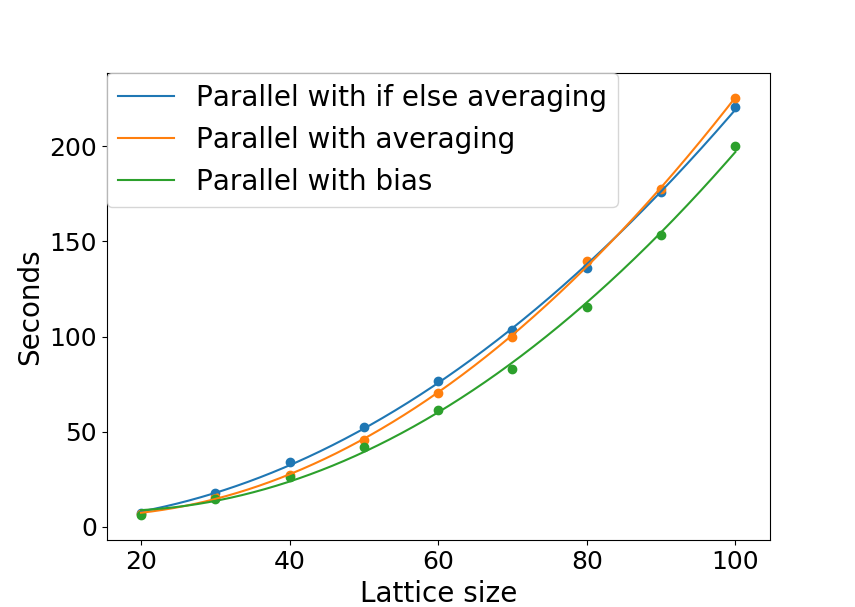
\includegraphics[keepaspectratio,height=10cm, width=10cm]{Projects/P04/parallel_comp.png}
  \caption{The orange line is parrallel model averaging with if-else test for the boundary conditions, the blue line is parallel model averaging (boundary matrix), and the green is parallel (boundary matrix) with bias. Tested on a laptop with Intel Core i7-7500 CPU 2.70GHZ. The solid lines are fitted with least square with second order polynomial.}
  \label{parallel_comp}
\end{figure}


\begin{figure}[H]
  \centering
  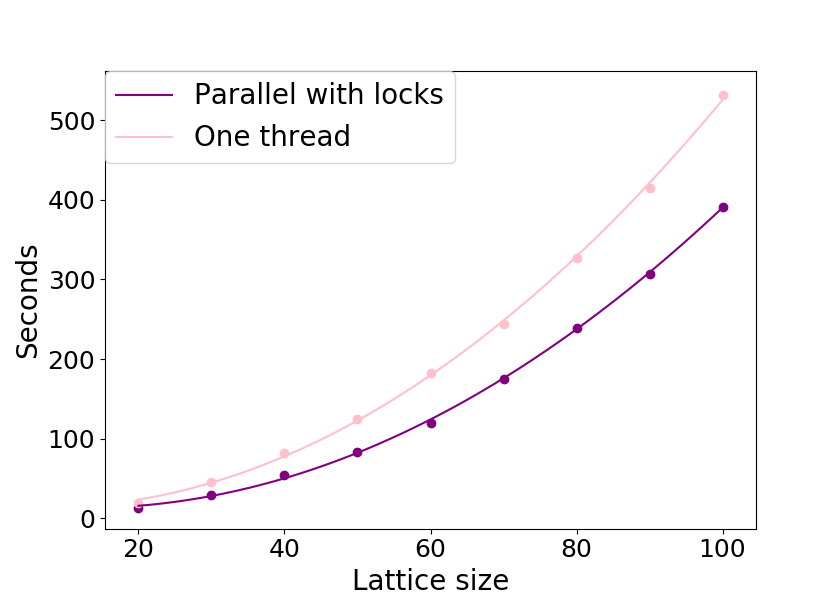
\includegraphics[keepaspectratio,height=10cm, width=10cm]{Projects/P04/Lock_vs_one.png}
  \caption{Parrallel with locks (boundary matrix) vs one thread (boundary matrix). Tested on a laptop with Intel Core i7-7500 CPU 2.70GHZ. The solid lines are fitted with least square with second order polynomial.}
  \label{Lock_vs_one}
\end{figure}






% \color{red}

% (ref) \url{https://www.researchgate.net/publication/2246795_Parallel_Simulation_of_the_Ising_Model}



% \begin{algorithm}[H]
% 	\caption{Metropolis algorithm for the simulation of Ising model. }
% 	\label{alg::metropolis}
% 	\KwIn{Size of the system $L$, temperature $T$, number of Monte Carlo cycles $MC$. }
% 	\KwOut{$\langle E \rangle$, $\langle E^2 \rangle$, $\langle |M| \rangle$, $\langle M^2 \rangle$, $C_V$ and $\chi$. } 
% 	Initialize spin lattice $a$ (in an ordered or random way)\;
% 	Calculate $E$, $E^2$, $|M|$, $M^2$ of the initial lattice\; 
% 	$E_{tot}=0,\,E^2_{tot}=0,\,|M|_{tot}=0,\,M^2_{tot}=0$\;
% 	\For{$i=1;i<=MC;i++$}
% 	{
% 		\For{$j=1;j<=L;j++$}
% 		{
% 			\For{$k=1;k<=L;k++$}
% 			{
% 				$r=$ a uniformly distributed random number in $[0,1]$\;
% 				Flip spin at position $(j,k)$\;
% 				Calculate the change of energy $\Delta E$\; 
% 				\If{$\Delta E < 0\ \mathrm{or}\ r<\exp\left(-\Delta E/T\right)$}
% 				{
% 					Accept this spin flip\; 
% 					Update $E$, $E^2$, $|M|$, $M^2$\;
% 				}
% 				\Else
% 				{
% 					Reverse this spin flip\;
% 				}
% 			Add $E$, $E^2$, $|M|$, $M^2$ to their corresponding ``tot" variables\; 
% 			}
% 		}
% 	}
% 	Calculate the average $\langle E \rangle$, $\langle E^2 \rangle$, $\langle |M| \rangle$, $\langle M^2 \rangle$ by dividing $L^2MC$\; 
% 	Calculate $C_V$ and $\chi$ by Eq. \ref{eq:cv} and \ref{eq:chi}\;
% \end{algorithm}
\color{black}


















\subsection{Unit tests}

We implemented three unit tests. One to check that the random number generator picked different numbers, and one for each of the ways we coded the boundary conditions. We printed out running results to see if the code was working, and did comparisons with the benchmark results, for the 2 $\times$ 2 system. %The reason we was not able to make more constructive unit test was down to the wish of making a highly efficient code. Due to that, we had to move a lot of the code around to see if there was possibilities of make the algorithms faster, and by that many of the smaller functions could not be tested out until we found out where to put them. We ended up with most of the algorithms in to one stand alone function.



\section{Results and discussions}
In this section we present and discuss the results of the Monte Carlo (MC) simulation of the 2D Ising model. Throughout the analysis, we assume the external magnetic field strength to be zero. We start our analysis by comparing our numerical simulation results with known exact analytical results. Then, for a finite lattice size, we illustrate how the expected values of the Ising model properties vary with time (MC cycles). Finally, we explore the second-order phase transition in the 2D Ising model.

\subsection{Benchmark}
To benchmark our implementation of the Metropolis algorithm for simulating the 2D Ising model, we select a $2\times2$ lattice at a temperature of $T=1.0$ $J/k_B$ and compare the numerical results with the corresponding exact analytical solutions (see Table \ref{tab:2by2}). As the number of MC cycles increase, the difference between our numerical results and the exact analytical solutions become smaller. How close we are to the analytical values depend on the physical quantity we are looking at. The energy $\langle E \rangle$ and the absolute value of the magnetization $\langle |M| \rangle$ expectation values approach their corresponding exact analytical values for relatively small MC cycles. However, we can observe that both the heat capacity $C_V$ and the magnetic susceptibility $\chi$ converge to their corresponding exact analytical values after a larger number of MC cycles. Nevertheless, to achieve an agreement with the exact analytical values to within three decimal places, we require $\sim 10^5$ MC cycles for both $\langle E \rangle$ and $\langle |M| \rangle$ while $C_V$ and $\chi$ each require $\sim 10^7$ MC cycles.

\begin{table}[H]
	\centering
	\begin{tabular}{ccccc}
		\hline
		\hline
		MC cycles & $\langle E \rangle$ & $\langle |M| \rangle$ & $C_V$ & $\chi$\\ 
		\hline
		$10^2$ & -2.0000000 & 1.0000000 & 0.0000000 & 0.0000000 \\ 
		$10^3$ & -1.9960000 & 0.9990000 & 0.0319360 & 0.0019960 \\ 
		$10^4$ & -1.9946000 & 0.9981000 & 0.0430834 & 0.0059856 \\ 
		$10^5$ & -1.9960000 & 0.9986650 & 0.0319360 & 0.0040029 \\ 
		$10^6$ & -1.9962320 & 0.9987585 & 0.0300872 & 0.0036748 \\
		$10^7$ & -1.9960404 & 0.9986834 & 0.0316173 & 0.0039333 \\
		$10^8$ & -1.9960001 & 0.9986654 & 0.0319397 & 0.0040006 \\
		$10^9$ & -1.9959819 & 0.9986607 & 0.0320838 & 0.0040110 \\
		Analytical & -1.9959821 & 0.9986607 & 0.0320787 & 0.0040107 \\
		\hline
		\hline 
	\end{tabular} 
	\caption{MC simulation with the Metropolis algorithm for a $2\times2$ lattice at a temperature of $T=1.0 J/k_B$. The corresponding analytical values are provided for benchmark. }
	\label{tab:2by2}
\end{table}

\subsection{Equilibration}
After benchmarking our implementation of the Metropolis algorithm, we now would like to use it to analyse some of the properties of the 2D Ising model. To extract useful information about the properties at a given temperature, we first have to run our simulation for many MC cycles (long period of time) until the system reaches equilibrium at the temperature we are interested in. This period of time (MC cycles) is known as the \textit{equilibration time}. After the system reaches equilibrium, we can extract the necessary physical properties by running our simulation for another several MC cycles and performing expectation over these MC cycles.

It is pertinent to notice that a system at equilibrium spends most of its time (MC cycles) in a small subset of states \cite{newmanb99}. Thus, its physical properties, like the energy and magnetization occupy only a narrow range of values. Moreover, at equilibrium the free energy of the system is at its minimum and the physical quantities we observe become roughly constant. Figure \ref{Energy_Mom_equilibration} shows for a $20\times20$ lattice, the mean energy and the mean absolute value of the magnetization as a function of the MC cycles (time). When $T=1.0 J/k_B$, with a disordered initialization, both the energy and the absolute magnetization reached equilibrium after $\sim 10^5$ MC cycles while for $T=2.4 J/k_B$ we need only $\sim10^4$ MC cycles.

To distinguish whether a system has reached the true equilibrium or is stuck in a local energy minimum, one should perform at least two different simulations of the same system, starting from different initial states. For our 2D Ising model, we initiate the system using ordered and random spin configurations. From Figure \ref{Energy_Mom_equilibration} we can observe that both the mean energy and absolute magnetization reach equilibrium at the same number of MC cycles and they both stay roughly constant after that. Here, ordered spin configuration implies all the spins in the lattice point towards the same direction, which is the equilibrium state at $T=0$. Moreover, a random spin configuration signifies an equilibrium state at $T=\infty$. Another observation we can make from Figure \ref{Energy_Mom_equilibration} is that when $T<<T_c$ and the system is initiated with an ordered state, the system reaches equilibrium after a few MC cycles. This is intuitively expected because for $T<<T_c$ the equilibrium state is close to an ordered state.

\begin{figure}[H]
  \centering
  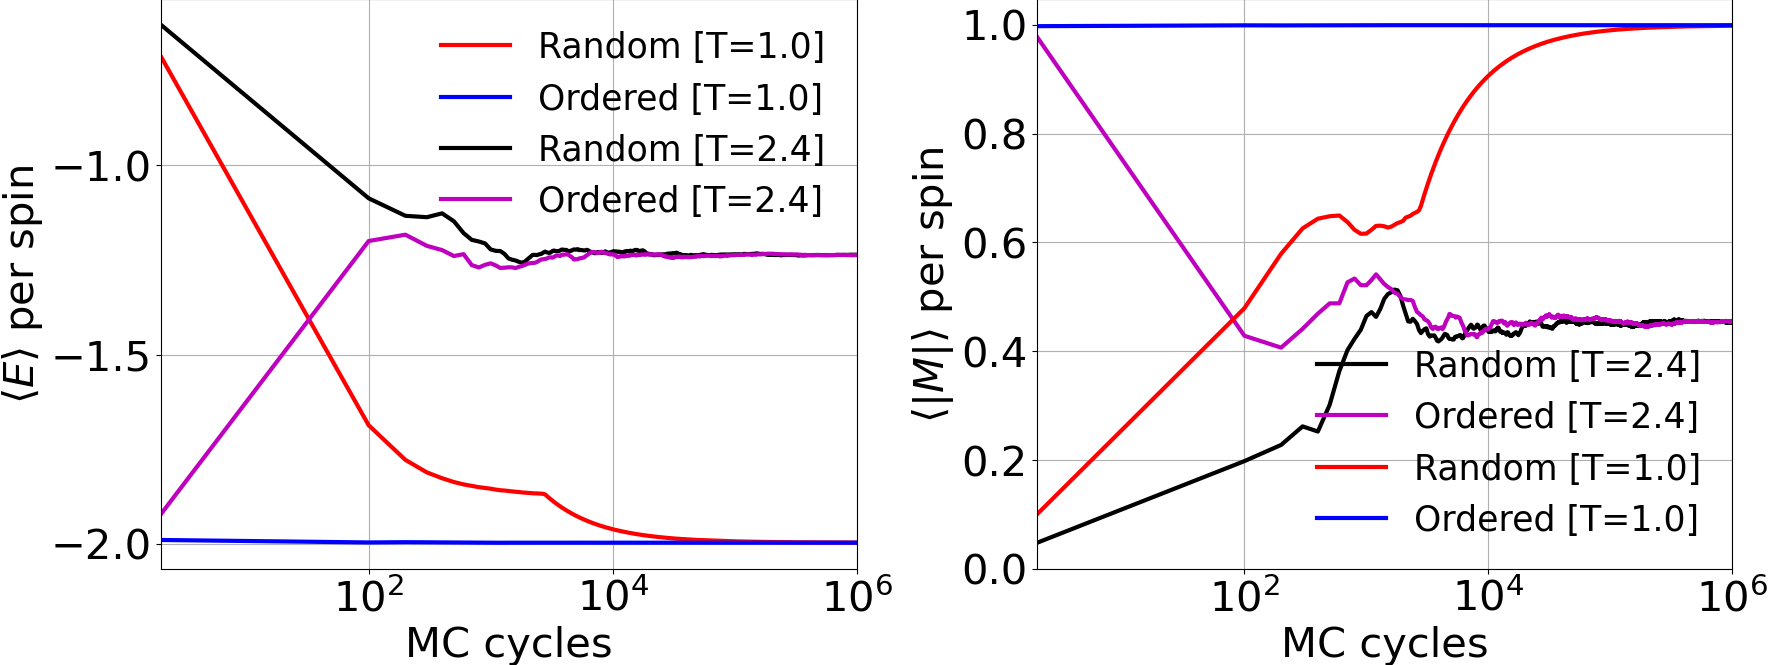
\includegraphics[keepaspectratio,height=10cm, width=12cm]{Projects/P04/Energy_Mom_equilibration.png}
  \caption{The mean energy $\langle E \rangle$ per spin (left) and the mean absolute value of magnetization $\langle |M| \rangle$ per spin (right) as a function of time (MC cycles) for a lattice size of $20\times20$. We consider two different temperatures, $T=1.0 J/k_B$ and $T=2.4 J/k_B$, and two ways of initializing our simulation, random and ordered.}
   \label{Energy_Mom_equilibration}
\end{figure}

We now consider how the number of accepted configurations (states) vary as a function of the MC cycles. Recalling the acceptance rule of the Metropolis algorithm, a chosen spin is flipped every time when $\Delta E < 0$, that is, when it would lower the energy of the system. A transition to a higher energy state is allowed with a probability governed by the Boltzmann factor $\exp\left(-\Delta E/T\right)$ when $\Delta E > 0$. Consequently, we see that at low temperatures ($T<<T_c$) this factor is small, so the probability of accepting a spin flip to a higher energy state is very low. In contrast, for higher temperatures the chance of accepting a spin flip becomes higher, see Figure \ref{accept_Temp}.

From Figure \ref{accept_NMC} we see that as the system reaches equilibrium at low temperatures the system resists change, whereas at higher temperatures the system is more likely to accept a proposed flip.  

\begin{figure}[H]
  \centering
  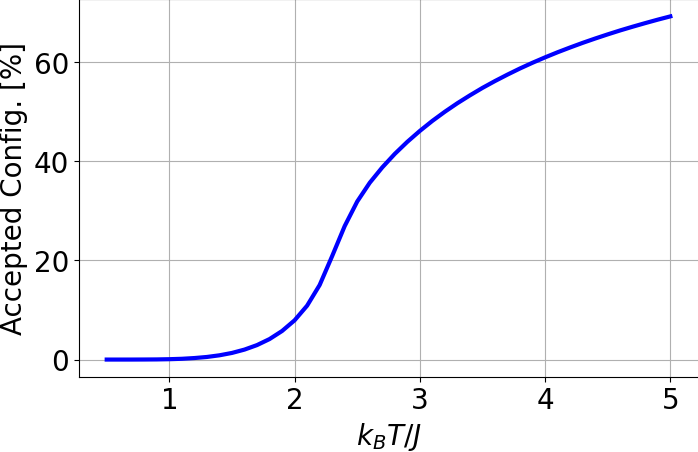
\includegraphics[width=0.7\textwidth]{Projects/P04/accept_Temp.png}
  \caption{The number of accepted configurations in percentile as a function of temperature. For each temperature we have run $10^6$ MC cycles.}
   \label{accept_Temp}
\end{figure}

\begin{figure}[H]
  \centering
  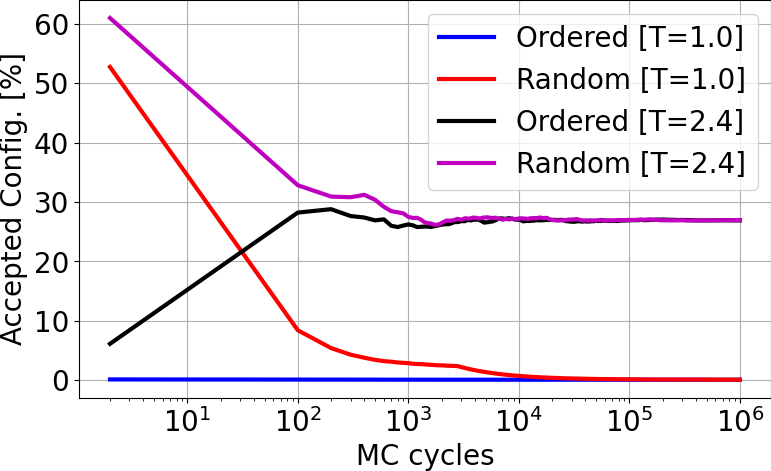
\includegraphics[width=0.7\textwidth]{Projects/P04/accept_NMC.png}
  \caption{The number of accepted configurations in percentile as a function of MC cycles for a lattice size of $20\times20$. We consider two different temperatures, $T=1.0J/k_B$ and $T=2.4J/k_B$, and two ways of initializing our simulation, random and ordered. }
   \label{accept_NMC}
\end{figure}





Lets now look at the energy distribution for a $20\times20$ lattice at two temperatures $1.0J/k_B$ and $2.4J/k_B$. Notice, the latter case is above the critical temperature while the first case is below the critical temperature. We have computed the probability distribution by counting the number of times a given energy appears in our simulation. All the energy counting is performed after the system reached its steady state. Figure \ref{energy_dist} shows the energy distribution histogram for temperature above and below the critical temperature. For the temperature below the critical value, we have an energy distribution that has small variance. In contrast, for the temperature above the critical value, we have an energy distribution that has relatively large variance. The main reason for having different distribution is that, for the higher temperature, we have higher chance of accessing different energies while for the lower temperature the equilibrium state has a  very low probability of flipping a spin, resulting in the same energy occurring many times. To quantify our analysis, we have computed the variance for the two cases and obtained a value of $0.03$ and $8.06$ for $T=1J/k_B$ and $T=2.4J/k_B$ respectively, for the entire $20 \times 20$ system. 



\begin{figure}[H]
  \centering
  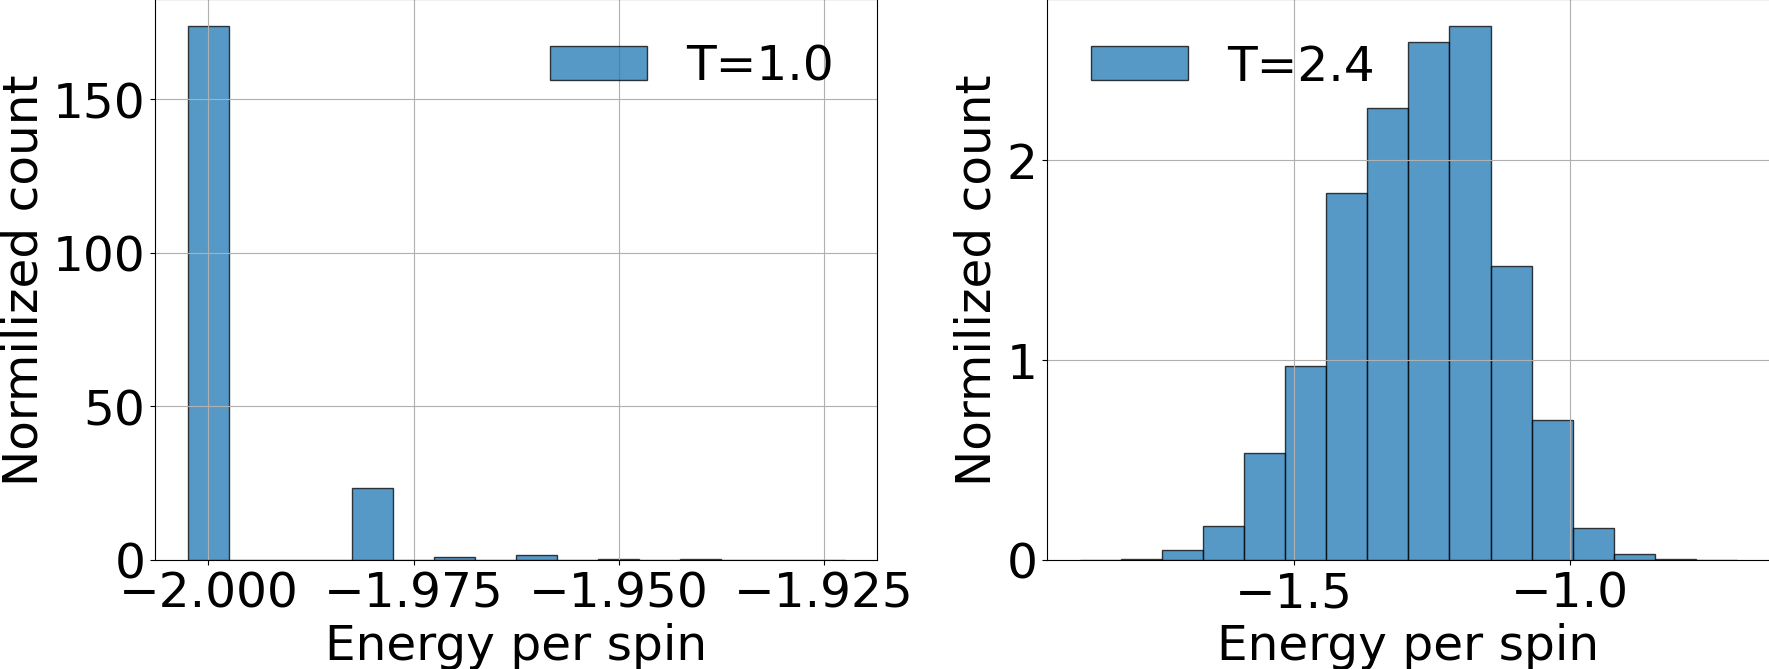
\includegraphics[width=1.0\textwidth]{Projects/P04/energy_dist.png}
  \caption{Histogram of the energy distribution, per spin, for a $20\times20$ lattice at two different temperatures of $1J/k_B$ and $2.4J/k_B$. Here, we have used $10^6$ MC cycles, but we started counting after $10^5$ MC cycles. Notice, we have used $20$ bins for both low and high temperature cases.}
   \label{energy_dist}
\end{figure}

\subsection{Second-order phase transitions}
This section is devoted to using MC simulation with the Metropolis algorithm on a 2D Ising model and extracting information about the second-order phase transition. Such a system has one crucial advantage that
its properties in the thermodynamic limit has exact analytical solutions \cite{PhysRev.65.117}. Thus, comparing our finite size lattice numerical simulations with the exact solution will allow us to have a feel for the sort of accuracy one can expect to achieve using the MC method. We have selected to run our simulation for a square lattice size of $20\times20$, $40\times40$,$60\times60$, $80\times80$, and $100\times100$. We initiate all the simulations with a random spin configuration and ran the simulations for $10^6$ MC cycles and at temperatures from $T = 2.0$ to $T = 2.5$ in steps of $0.01$. The equilibration time for our simulation is estimated from the results in Figure \ref{Energy_Mom_equilibration}. Note that we only used one lattice size, and that we are working under the assumption that the calculations hold for larger lattice sizes. Using these parameters we can now calculate the equilibrium properties of the 2D Ising model for different finite size lattices.

The first property we have looked at is the mean energy per spin. Figure \ref{Energy_sptr} shows the result for different finite size lattices. Here, we can observe that at the critical temperature the energy curves have an inflection point, where the slope of the energy curve changes its sign. Moreover, the lager the lattice size the more abrupt the slope change and it is easier to identify the inflection point where we have the critical temperature. The energy per spin approaches a value of $-2J$ for $T << T_c$ and for $T>>T_c$ it approaches a value of zero.

\begin{figure}[H]
  \centering
  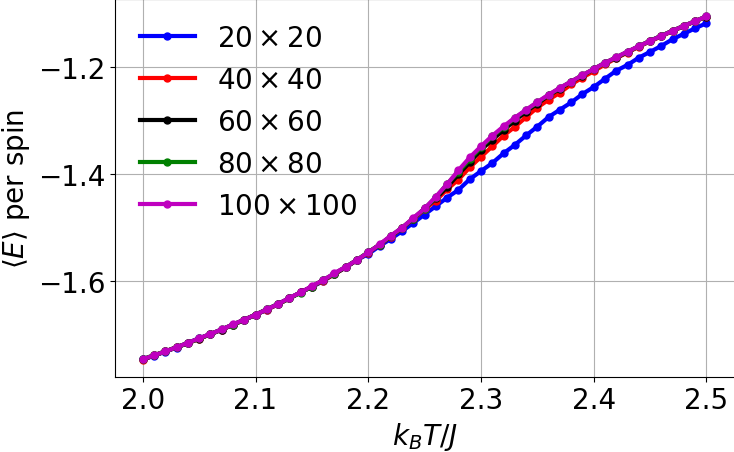
\includegraphics[width=1.0\textwidth]{Projects/P04/Energy_sptr.png}
  \caption{Thermal average of the energy versus temperature for the Ising model on a $20\times20$, $40\times40$, $60\times60$, $80\times80$, and $100\times100$ square lattices.}
   \label{Energy_sptr}
\end{figure}

From thermodynamics \cite{giordano}, we know that the specific heat ($C_V$) is proportional to the derivative of the energy with respect to temperature. Thus, at the critical temperature, we expect the specific heat to diverge in the thermodynamic limit. For a finite size lattice, however, the specific heat has a finite value at the critical temperature. Although it is possible to compute $C_V$ by taking the derivative of the average energy with respect to temperature, here we have used fluctuation-dissipation theorem of statistical mechanics \cite{giordano} and derived $C_V$ as the ratio between the variance of the energy and the square of the temperature. Figure \ref{Cv_sptr} shows the behaviour of $C_V$ for different finite size square lattices. As expected, $C_V$ has a peak in the vicinity of $T_c$. This peak value increases in magnitude and gets closer to the analytical value of $T_c$ as the size of the square lattice gets larger.

\begin{figure}[H]
  \centering
  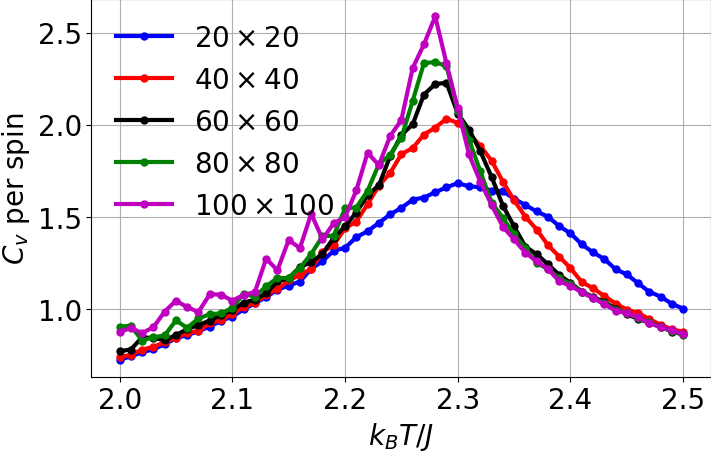
\includegraphics[width=1.0\textwidth]{Projects/P04/Cv_sptr.png}
  \caption{The heat capacity as a function of temperature computed after $10^6$ MC cycles and using the fluctuation-dissipation relation for $20\times20$,$40\times40$,$60\times60$,$80\times80$,and $100\times100$ square lattices.}
   \label{Cv_sptr}
\end{figure}

Magnetization is an order parameter of the Ising model \cite{newmanb99}. An order parameter has a zero value on one side of a phase transition and non-zero on the other. Here, we analyse the mean absolute value of the magnetization for different finite size lattices. Figure \ref{Mom_sptr} shows the mean absolute magnetization per spin as a function of temperature. In the thermodynamic limit the mean absolute magnetization per spin for temperature above $T_c$ is zero. From our MC simulation of different finite size lattices, we can observe that the phase transition at $T_c$ gets sharper as the size of the lattice gets larger. Using the fluctuation-dissipation relation, we can compute the magnetic susceptibility $\chi$ as the ratio between the variance of the magnetization and temperature. Figure \ref{Chi_sptr} shows $\chi$ per spin as a function of temperature for different finite size lattices. We can observe that $\chi$ around $T_c$ has a peak value and this value gets larger and closer to the analytical $T_c$ as the size of the lattice gets larger.

\begin{figure}[H]
  \centering
  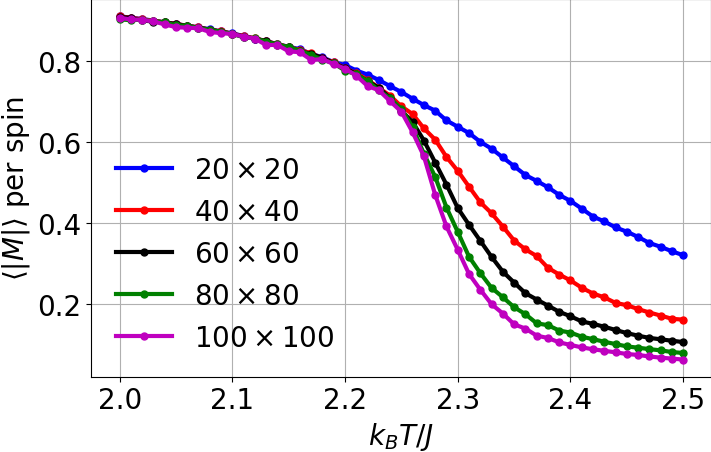
\includegraphics[width=1.0\textwidth]{Projects/P04/Mom_sptr.png}
  \caption{The mean magnitude of the magnetization per spin as a function of temperature the Ising model on a $20\times20$, $40\times40$, $60\times60$, $80\times80$, and $100\times100$ square lattices.}
   \label{Mom_sptr}
\end{figure}

\begin{figure}[H]
  \centering
  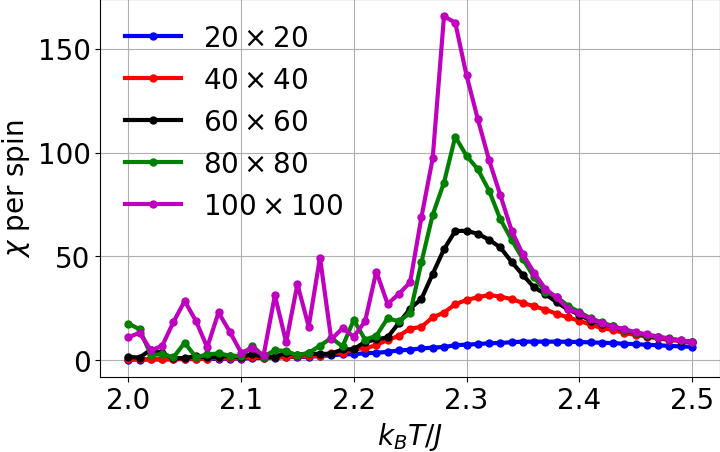
\includegraphics[width=1.0\textwidth]{Projects/P04/Chi_sptr.png}
  \caption{The susceptibility $\chi$ per spin as a function of temperature the Ising model on a $20\times20$, $40\times40$, $60\times60$, $80\times80$, and $100\times100$ square lattices.}
   \label{Chi_sptr}
\end{figure}

We now use the finite size scaling relations to find the critical temperature in the thermodynamic limit (infinite lattice size) from the information we have on finite size lattices. We first reformulate Equation \ref{eq:noe} as

\begin{equation}
  T_C(L) = T_C(L=\infty) + aL^{-1/\nu} \label{eq:noe2}.
\end{equation}
For $\nu=1$, we have a linear relationship between $T_C(L)$ and $L^{-1}$ with $T_C(L=\infty)$ being the intercept. Thus, we estimate the value of $T_C(L=\infty)$ by performing a least square fitting of the data extracted from the maximum of the $\chi$ versus $T$ plot in Figure \ref{Chi_sptr}. Consequently, the result of the linear regression is shown in Figure \ref{Chi_Tc} where we estimate $T_C(L=\infty)=2.2625 \pm 0.005$.

\begin{figure}[H]
  \centering
  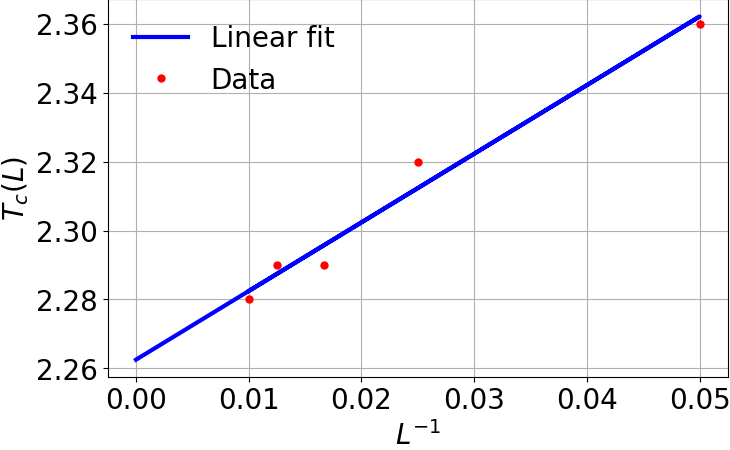
\includegraphics[width=1.0\textwidth]{Projects/P04/Chi_Tc.png}
  \caption{A plot showing the variation of temperature as a function of the inverse lattice size. The corresponding least square prediction is shown with a blue line.}
   \label{Chi_Tc}
\end{figure}

\section{Conclusion}
In this project we studied the 2D finite size Ising model using MC-based Metropolis algorithm. To avoid edge effects, we used periodic boundary conditions. The results of our simulation were benchmarked for a $2\times2$ lattice. The main requirement for producing accurate results were to consider large number of MC cycles so that the system reaches its equilibrium state. For a lattice size of $20\times20$, we analysed the number of MC cycles required for the system to reach equilibrium. For low temperatures, $T<T_c$, the system reaches equilibrium with a few hundreds of MC cycles when the simulation is initiated with ordered spin configuration. However, for high temperatures, $T>Tc$, the system reached equilibrium after $\sim 10^4$ MC cycles regardless of how we initialized the spin configuration. The Metropolis algorithm allowed us to calculate the properties of the Ising model without having to calculate the corresponding probability distribution. Nevertheless, counting the number of occurrences of energies and generating a histogram we have showed the energy variation at equilibrium follows the Boltzmann distribution. Finally, we run the Metropolis algorithm for different finite size lattices for temperatures between $2$ and $2.5$ using $10^6$ MC cycles. Different methods of parallelization where implemented, we concluded that the combination of compilation flags and parallelization with model averaging, speed the code up by approximately five times, on a computer with 12 available threads. The mean energy, absolute value of magnetization, heat capacity, and susceptibility of the 2D Ising model is analysed close to the critical temperature where second-order phase transition happens. Moreover, a finite size scaling analysis was undertaken to determine the
critical temperature at the thermodynamic limit using the results of finite size lattices. The accuracy of the result is very compelling and matches the theoretical value within the uncertainty of the result.

%\bibliographystyle{plain}
%\bibliographystyle{siam}
\bibliography{sample}
\bibliographystyle{IEEEtran}

\begin{appendix}
\newpage
\section{Model averaging distribution comparisons}
\label{section:Boxplots}

In the plots below we have compared the results from running model averaging against a single chain. From the top of in each plot we have 250k MC cycles, 500k MC cycles, 750k MC cycles, and 1 million MC cycles run on one thread, and the last one (the blue) is 250k cycles for each of the 4 threads available on our computer with their own systems and then averaging them. We simulated each one 30 times.


\subsection*{Mean Energy}

\begin{figure}[H]
  \centering
  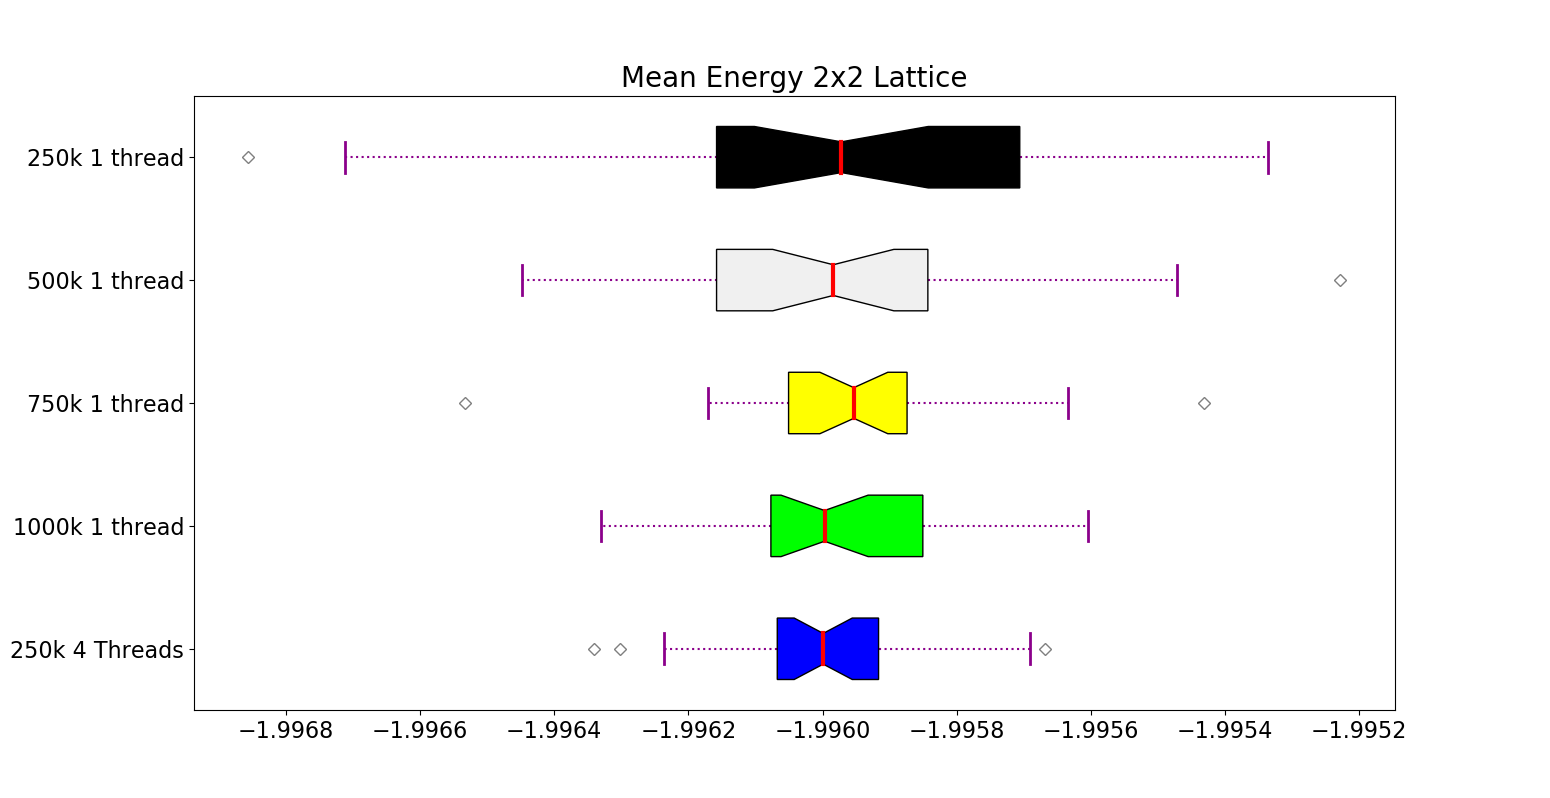
\includegraphics[width=1.2\textwidth]{Projects/P04/2x2_M_Energy.png}
  \caption{2x2 lattice mean Energy.}
  \label{2x2_M_Energy}
\end{figure}
\begin{figure}[H]
  \centering
  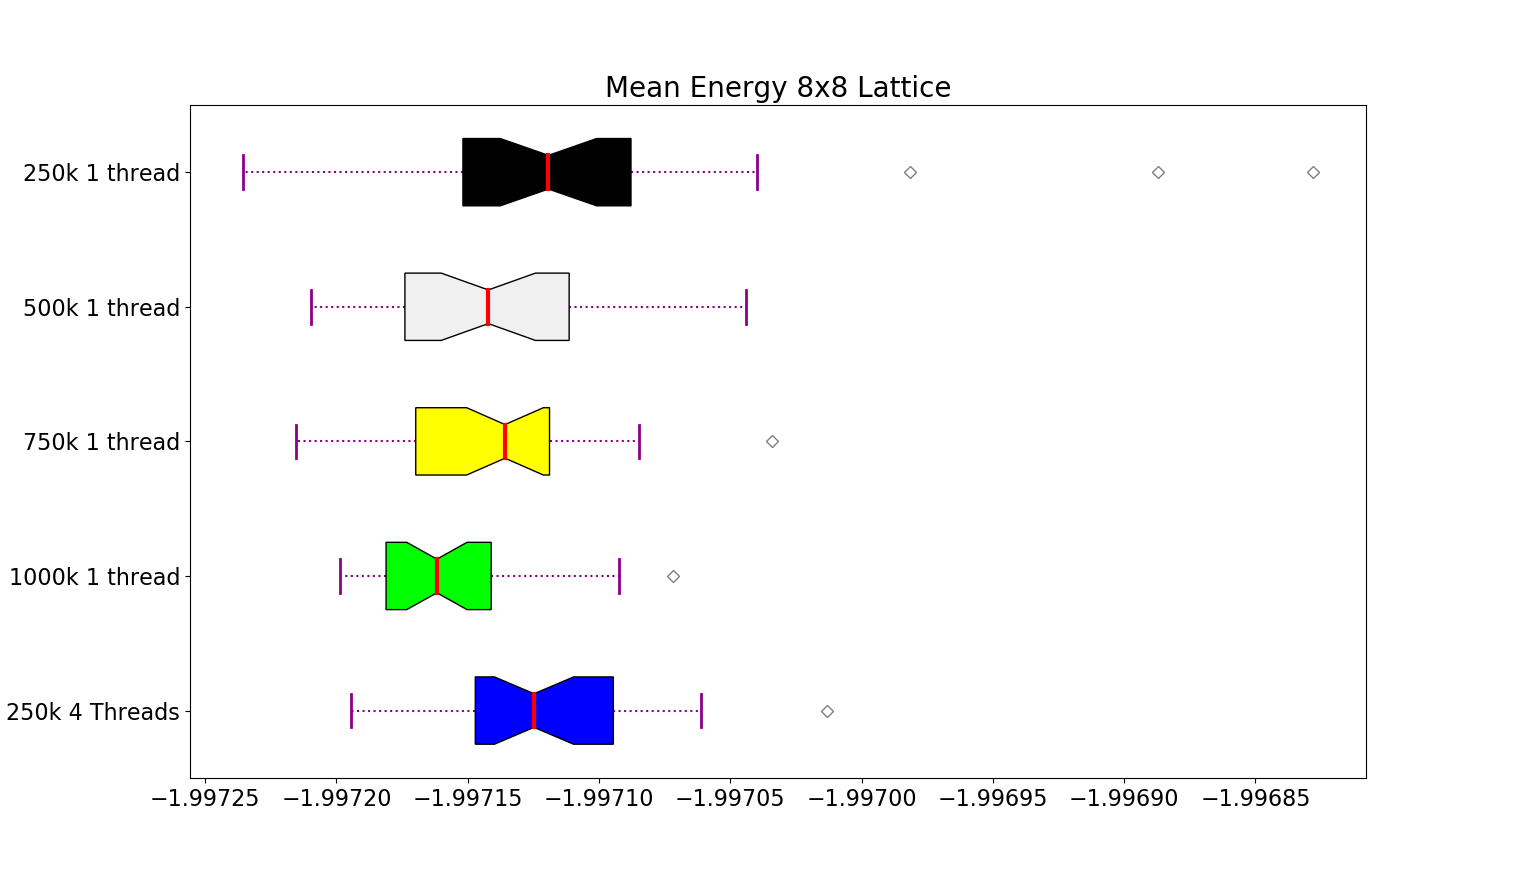
\includegraphics[width=1.2\textwidth]{Projects/P04/8x8_M_Energy.png}
  \caption{8x8 lattice mean Energy.}
  \label{8x8_M_Energy}
\end{figure}
\begin{figure}[H]
  \centering
  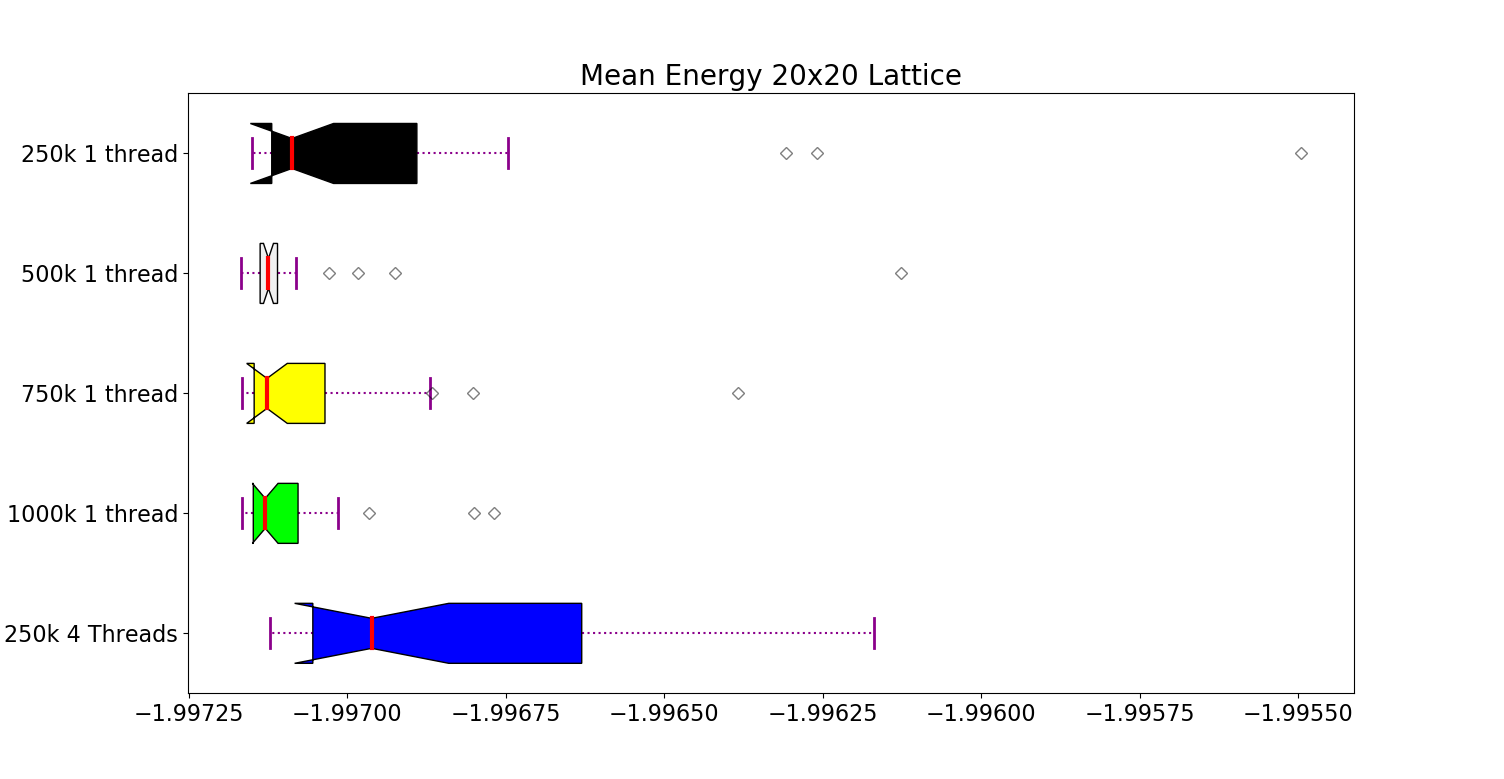
\includegraphics[width=1.2\textwidth]{Projects/P04/20x20_M_Energy.png}
  \caption{20x20 lattice mean Energy.}
  \label{20x20_M_Energy}
\end{figure}

% \subsection*{Energy squared}


% \begin{figure}[H]
%   \centering
%   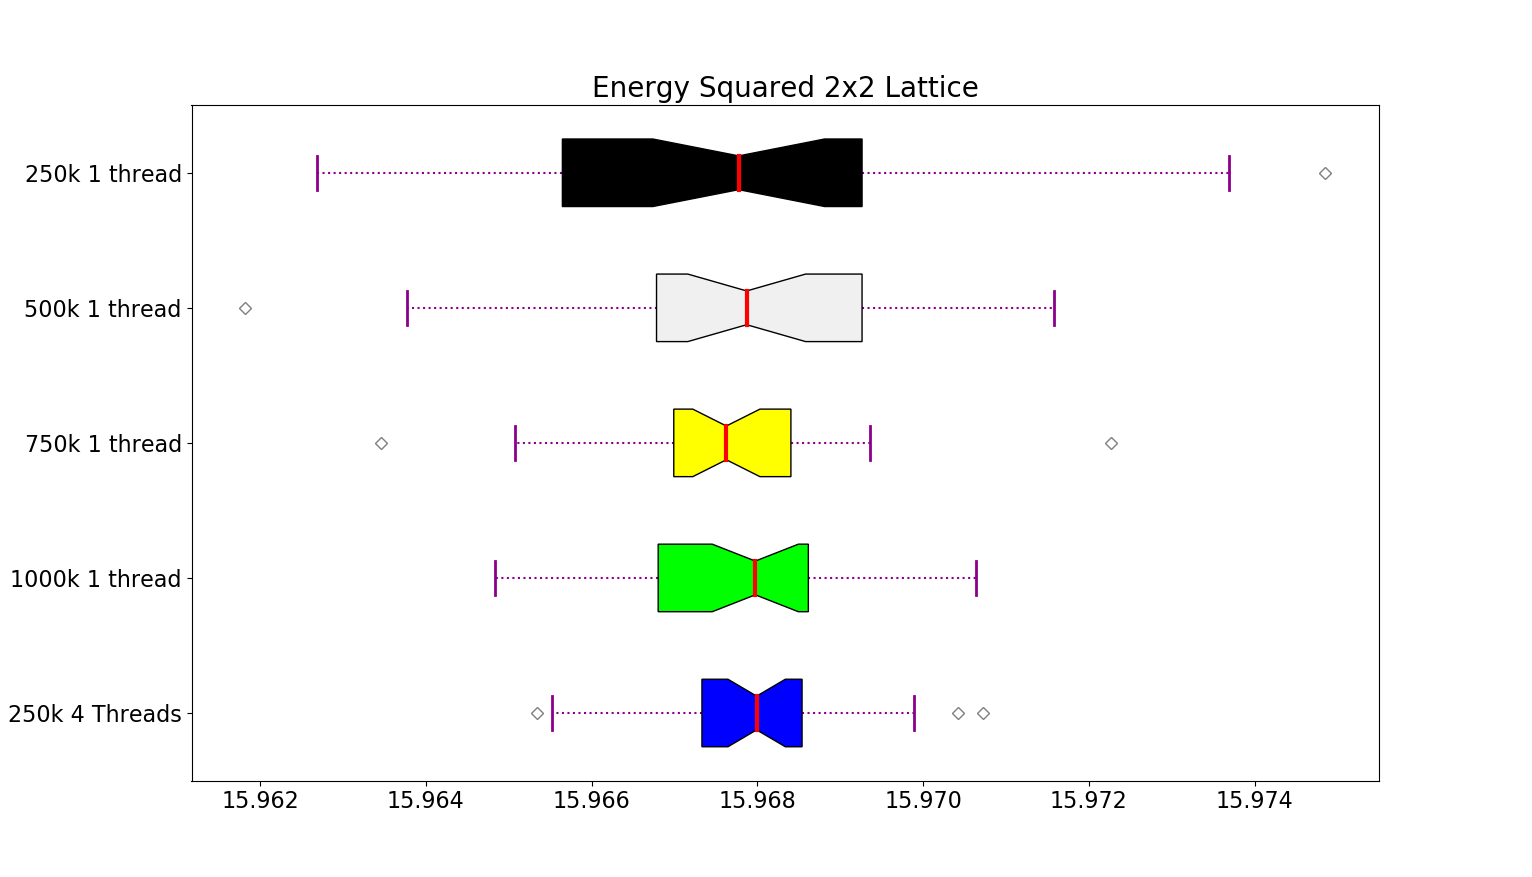
\includegraphics[width=1.0\textwidth]{Projects/P04/2x2_Energy_sq.png}
%   \caption{2x2 Energy squared.}
%   \label{2x2_M_Energy}
% \end{figure}
% \begin{figure}[H]
%   \centering
%   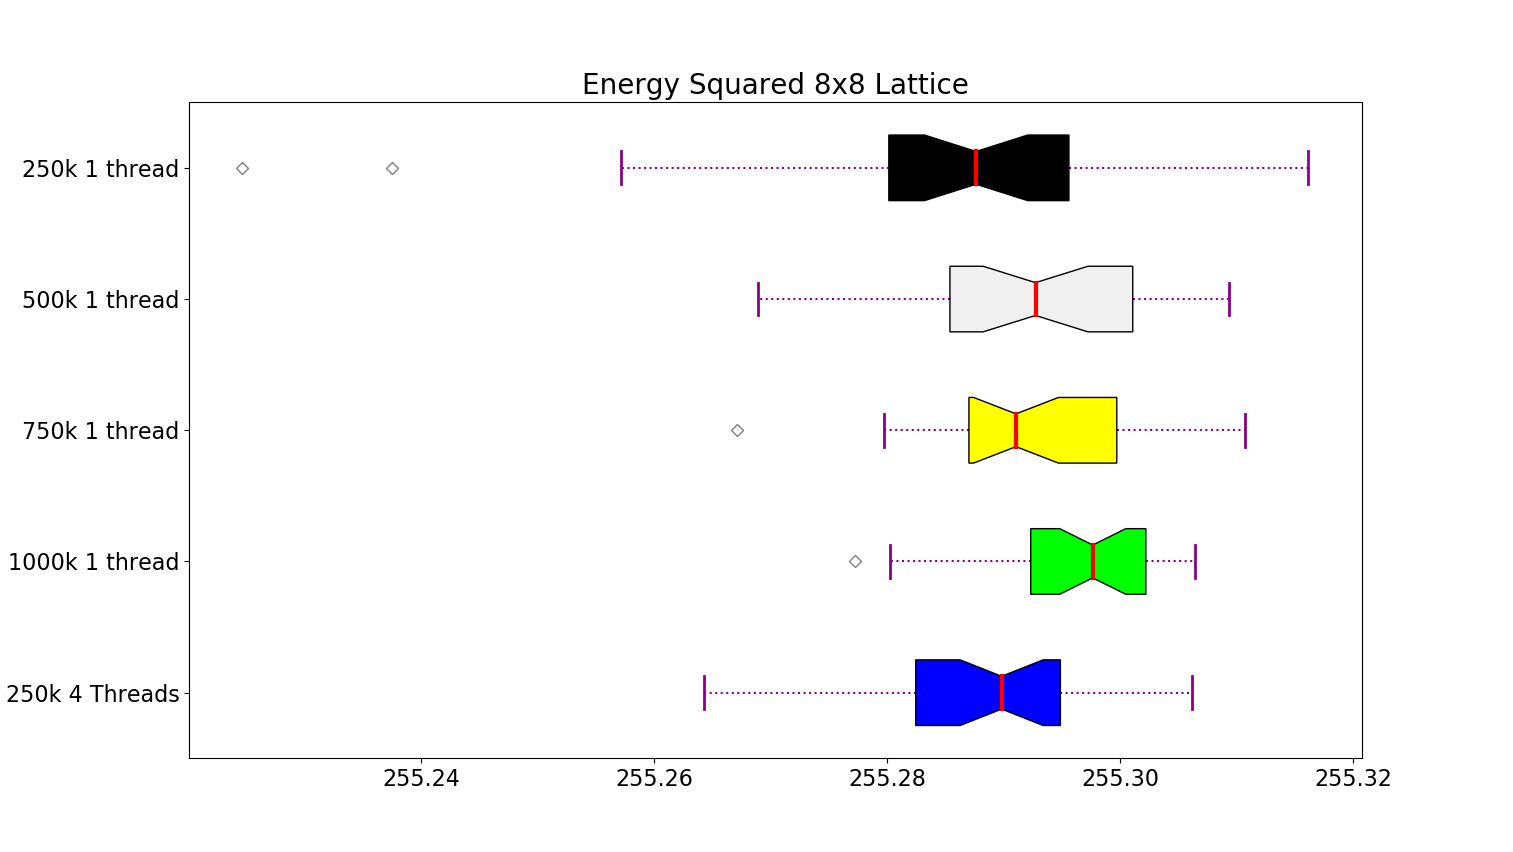
\includegraphics[width=1.0\textwidth]{Projects/P04/8x8_Energy_sq.png}
%   \caption{8x8 Energy squared.}
%   \label{8x8_Energy_sq}
% \end{figure}
% \begin{figure}[H]
%   \centering
%   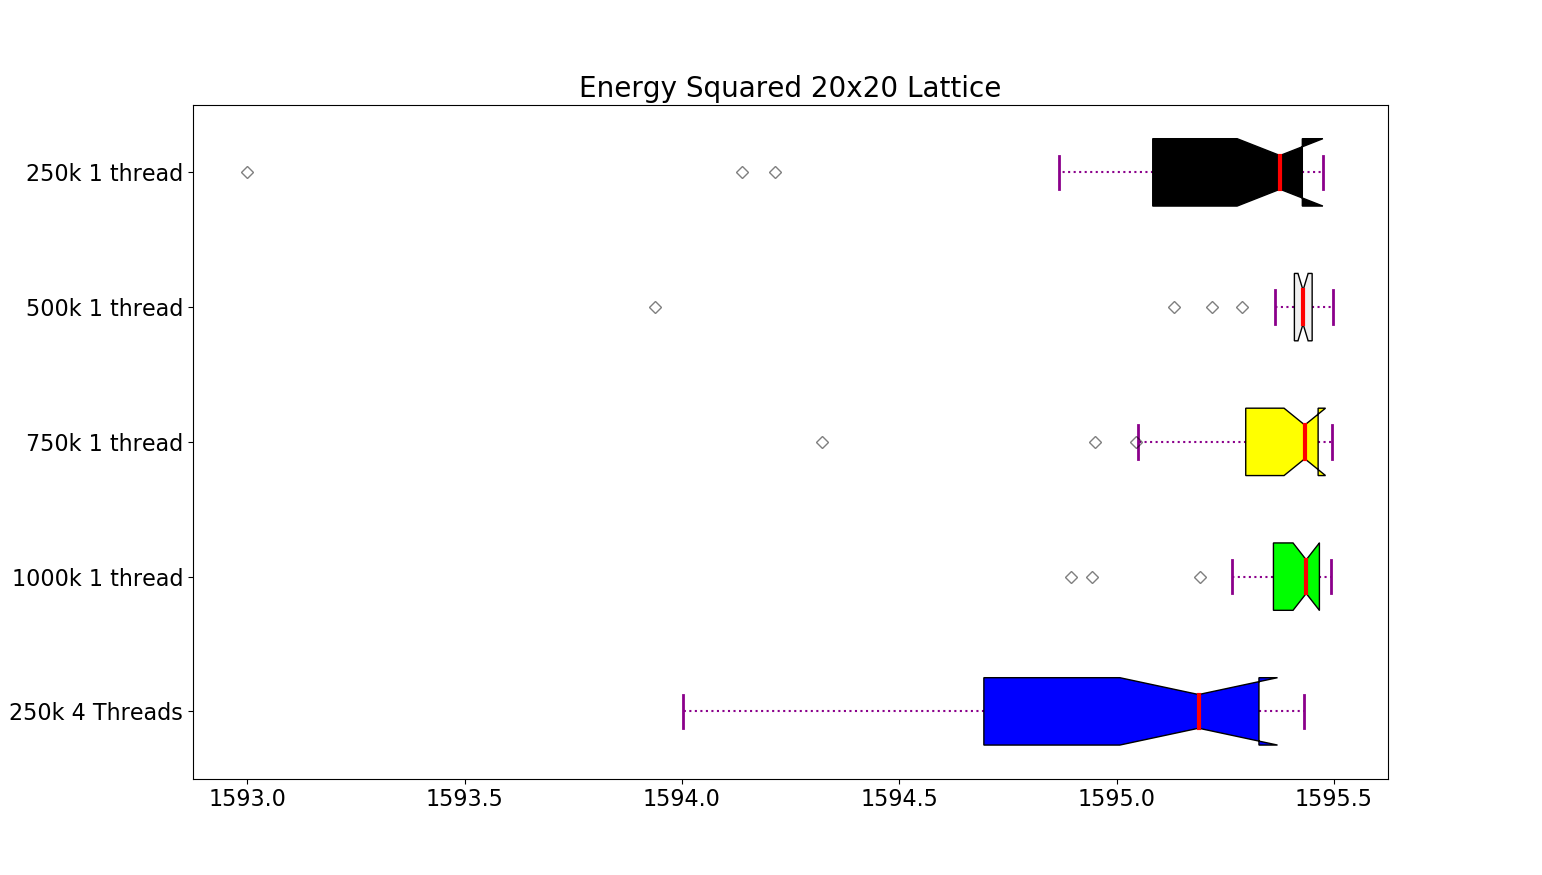
\includegraphics[width=1.0\textwidth]{Projects/P04/20x20_Energy_sq.png}
%   \caption{20x20 Energy squared.}
%   \label{20x20_Energy_sq}
% \end{figure}

\subsection*{Absolute Magnetization}


\begin{figure}[H]
  \centering
  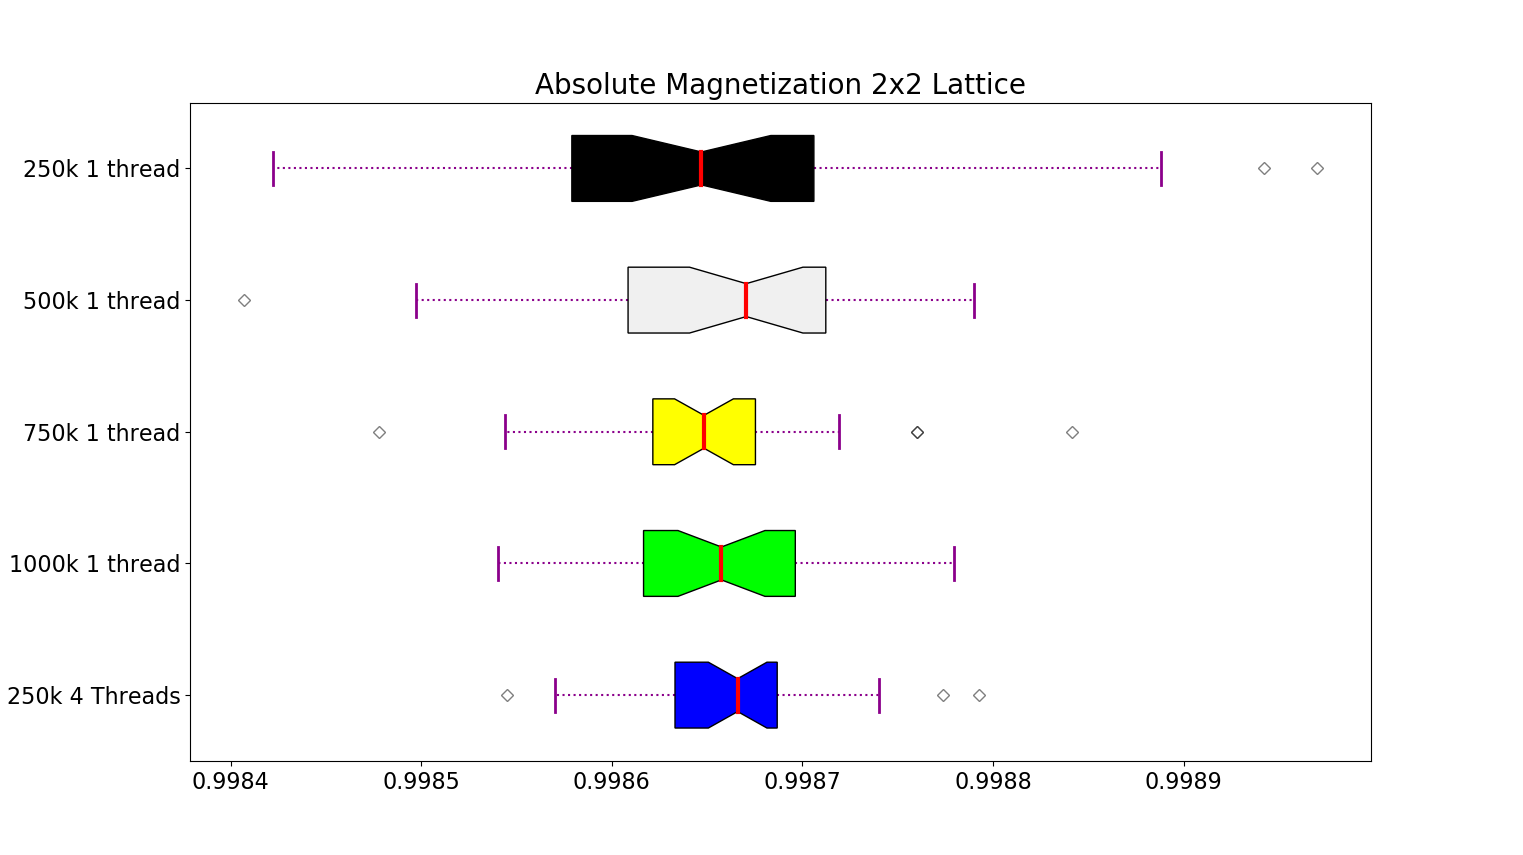
\includegraphics[width=1.2\textwidth]{Projects/P04/2x2_A_Mag.png}
  \caption{2x2 Absolute Magnetization.}
  \label{2x2_A_Mag}
\end{figure}
\begin{figure}[H]
  \centering
  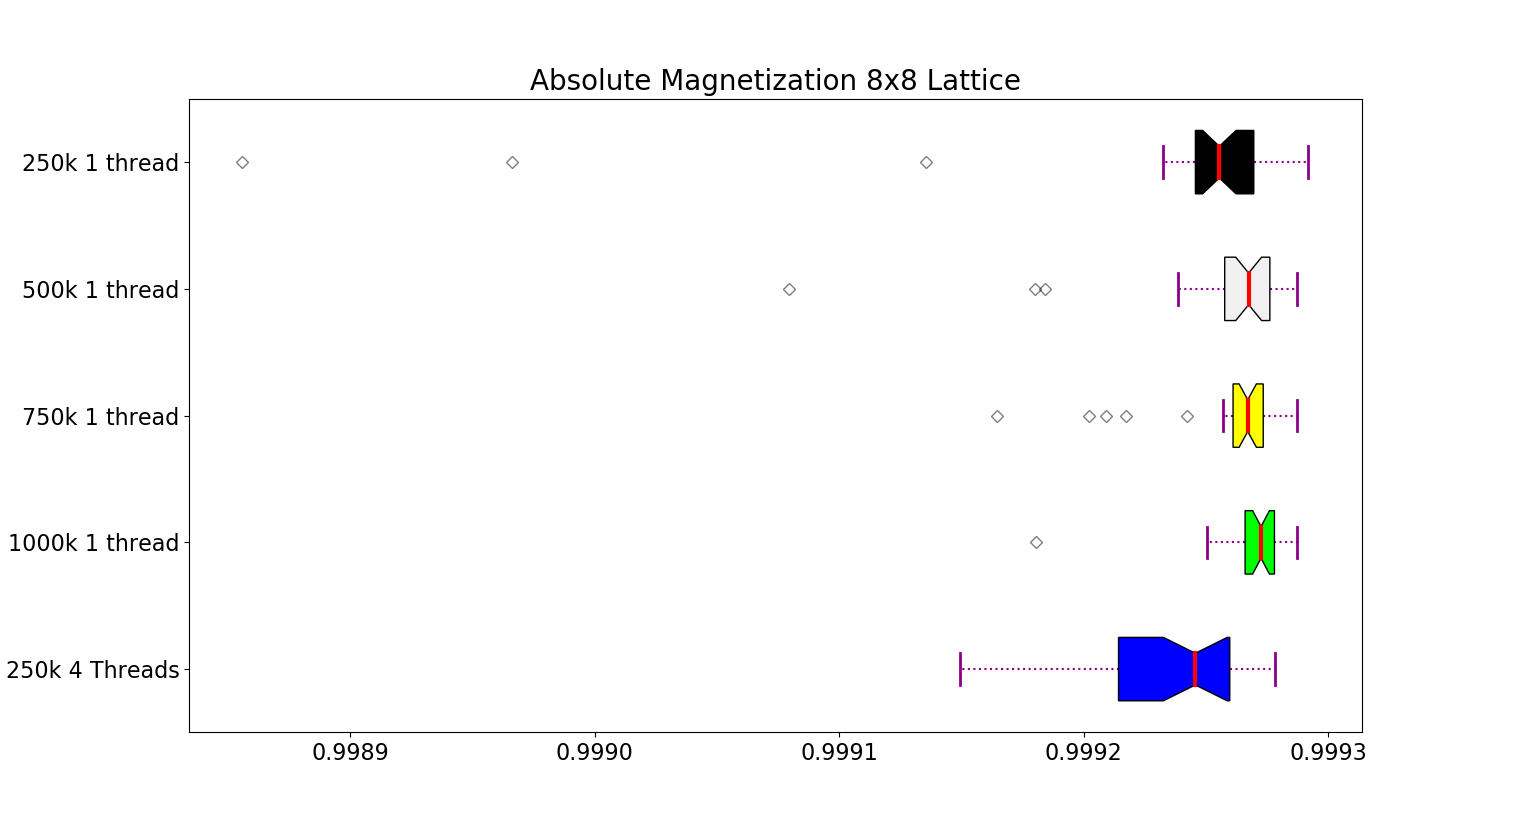
\includegraphics[width=1.2\textwidth]{Projects/P04/8x8_A_Mag.png}
  \caption{8x8 Absolute Magnetization.}
  \label{8x8_A_Mag}
\end{figure}
\begin{figure}[H]
  \centering
  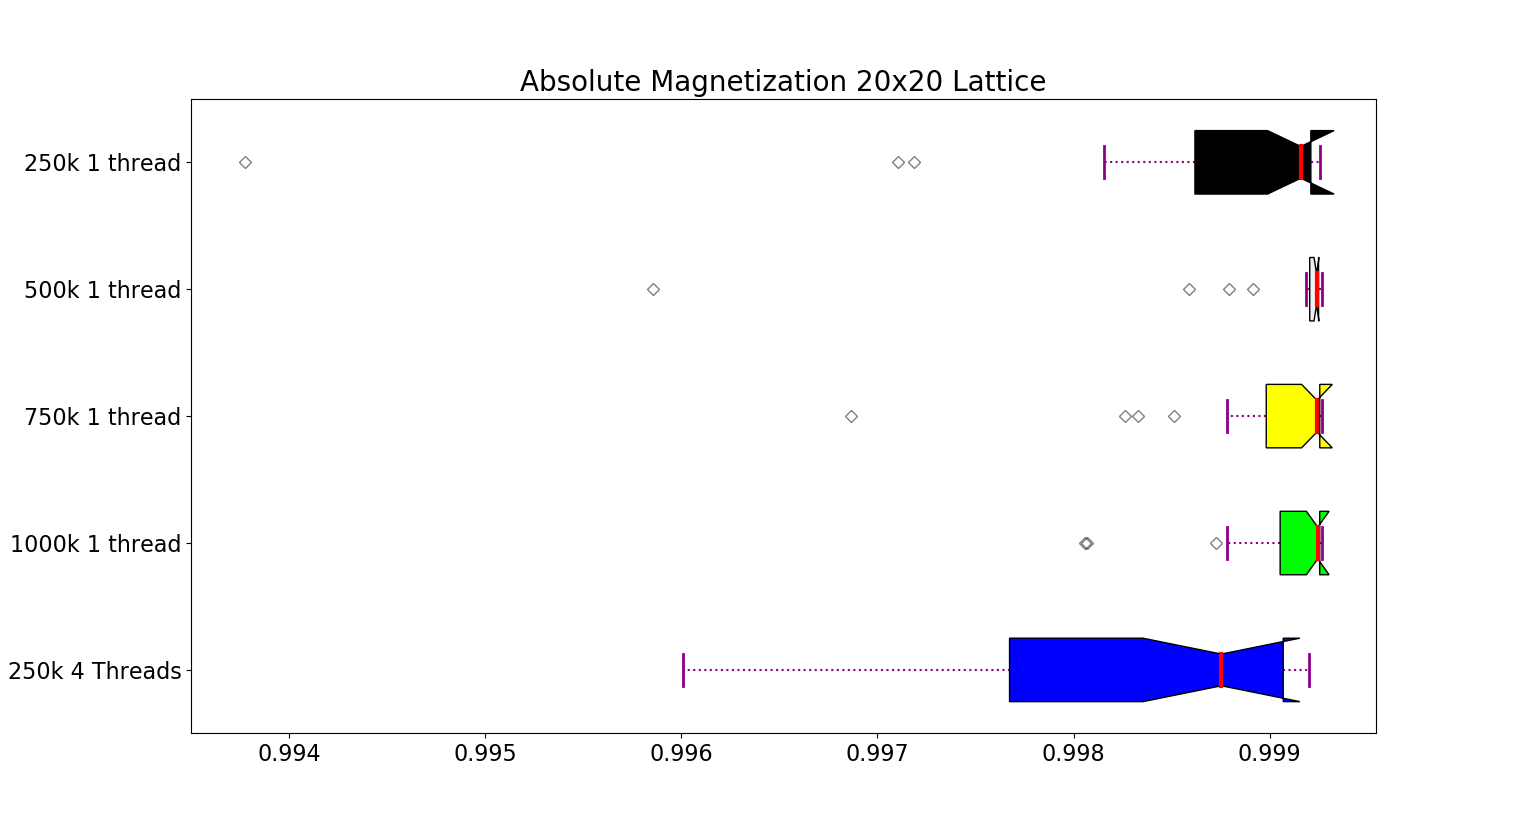
\includegraphics[width=1.2\textwidth]{Projects/P04/20x20_A_Mag.png}
  \caption{20x20 Absolute Magnetization.}
  \label{20x20_A_Mag}
\end{figure}

% \subsection*{Magnetization squared}


% \begin{figure}[H]
%   \centering
%   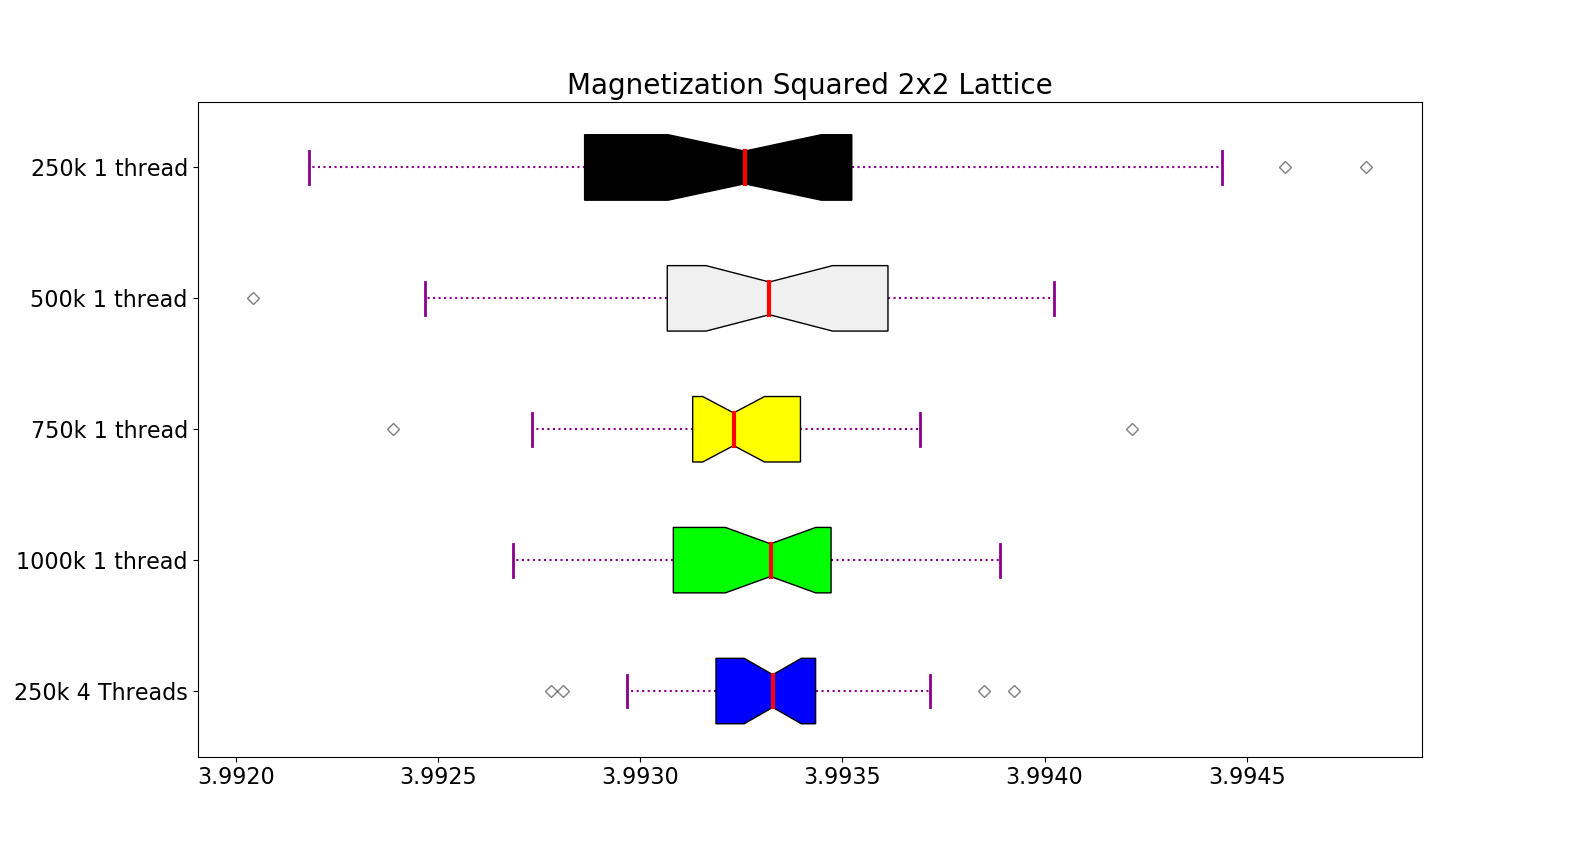
\includegraphics[width=1.0\textwidth]{Projects/P04/2x2_Mag_sq.png}
%   \caption{2x2 Magnetization squared.}
%   \label{2x2_Mag_sq}
% \end{figure}
% \begin{figure}[H]
%   \centering
%   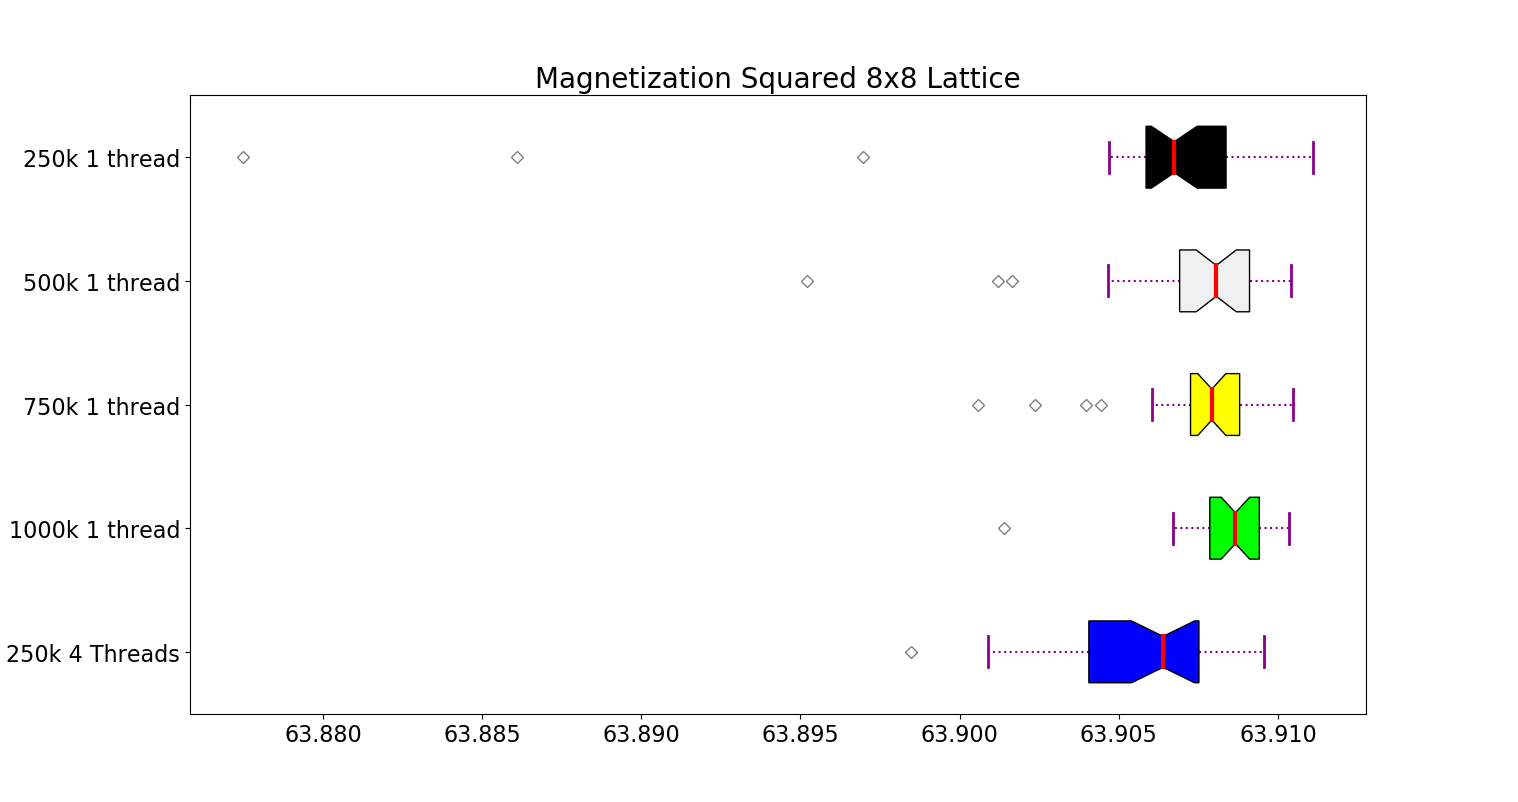
\includegraphics[width=1.0\textwidth]{Projects/P04/8x8_Mag_sq.png}
%   \caption{8x8 Magnetization squared.}
%   \label{8x8_Mag_sq}
% \end{figure}
% \begin{figure}[H]
%   \centering
%   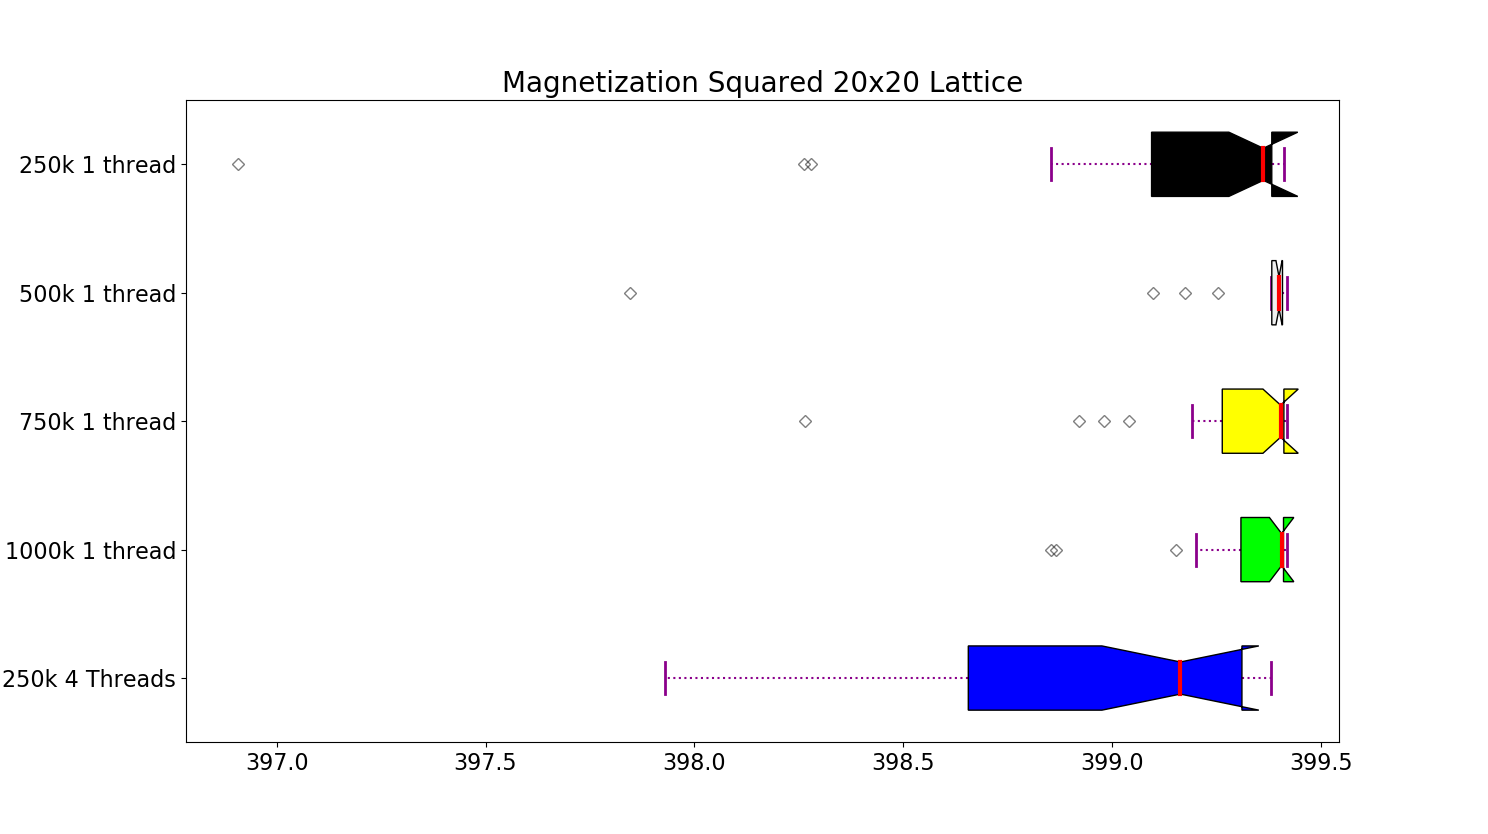
\includegraphics[width=1.0\textwidth]{Projects/P04/20x20_Mag_sq.png}
%   \caption{20x20 Magnetization squared.}
%   \label{20x20_A_Mag}
% \end{figure}


% \subsection*{Heat capacity}


% \begin{figure}[H]
%   \centering
%   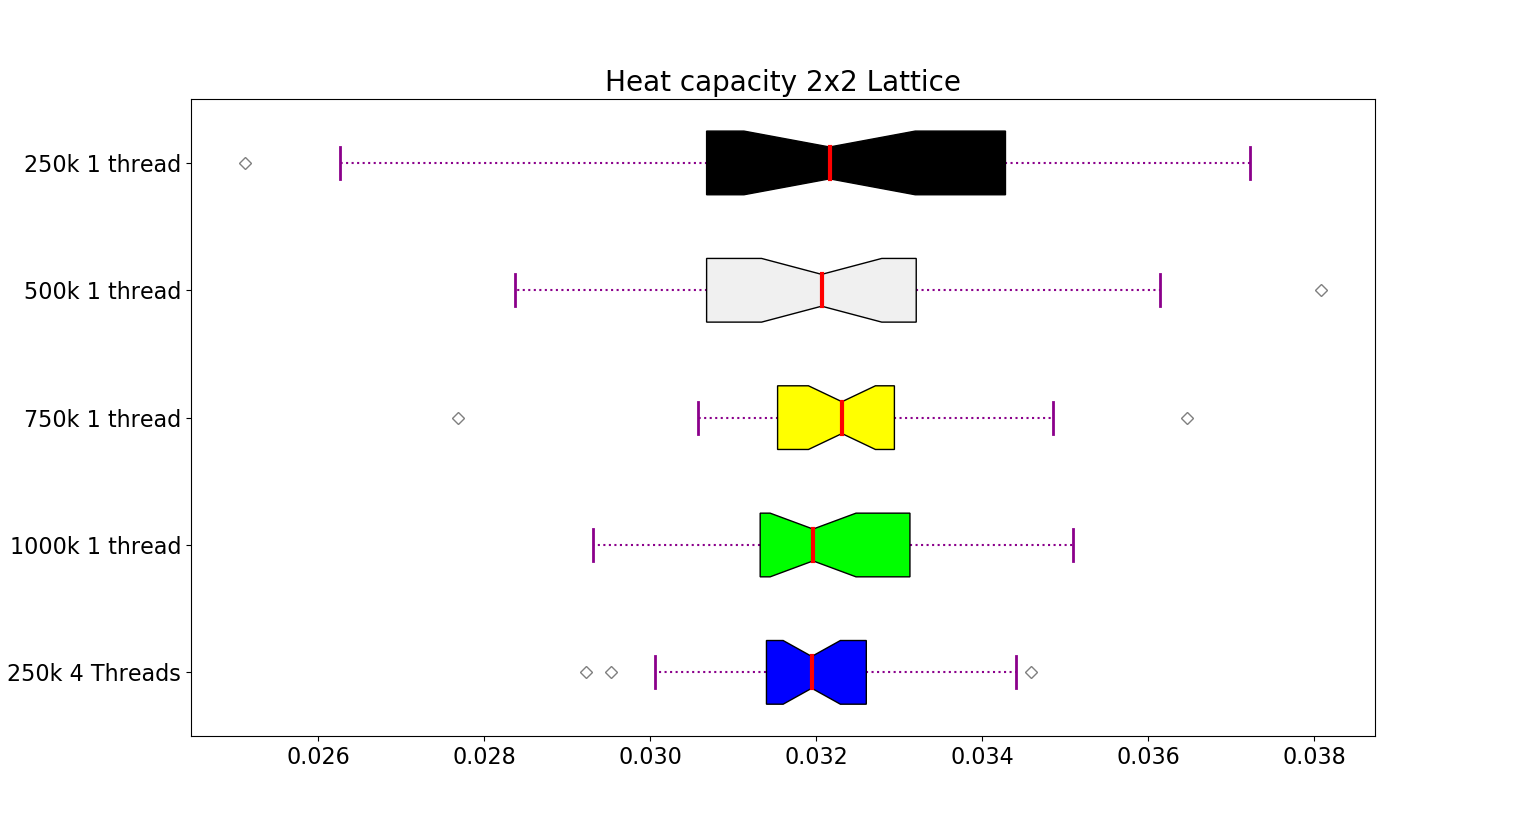
\includegraphics[width=1.0\textwidth]{Projects/P04/2x2_Cv.png}
%   \caption{2x2 Heat capacity.}
%   \label{2x2_Cv}
% \end{figure}
% \begin{figure}[H]
%   \centering
%   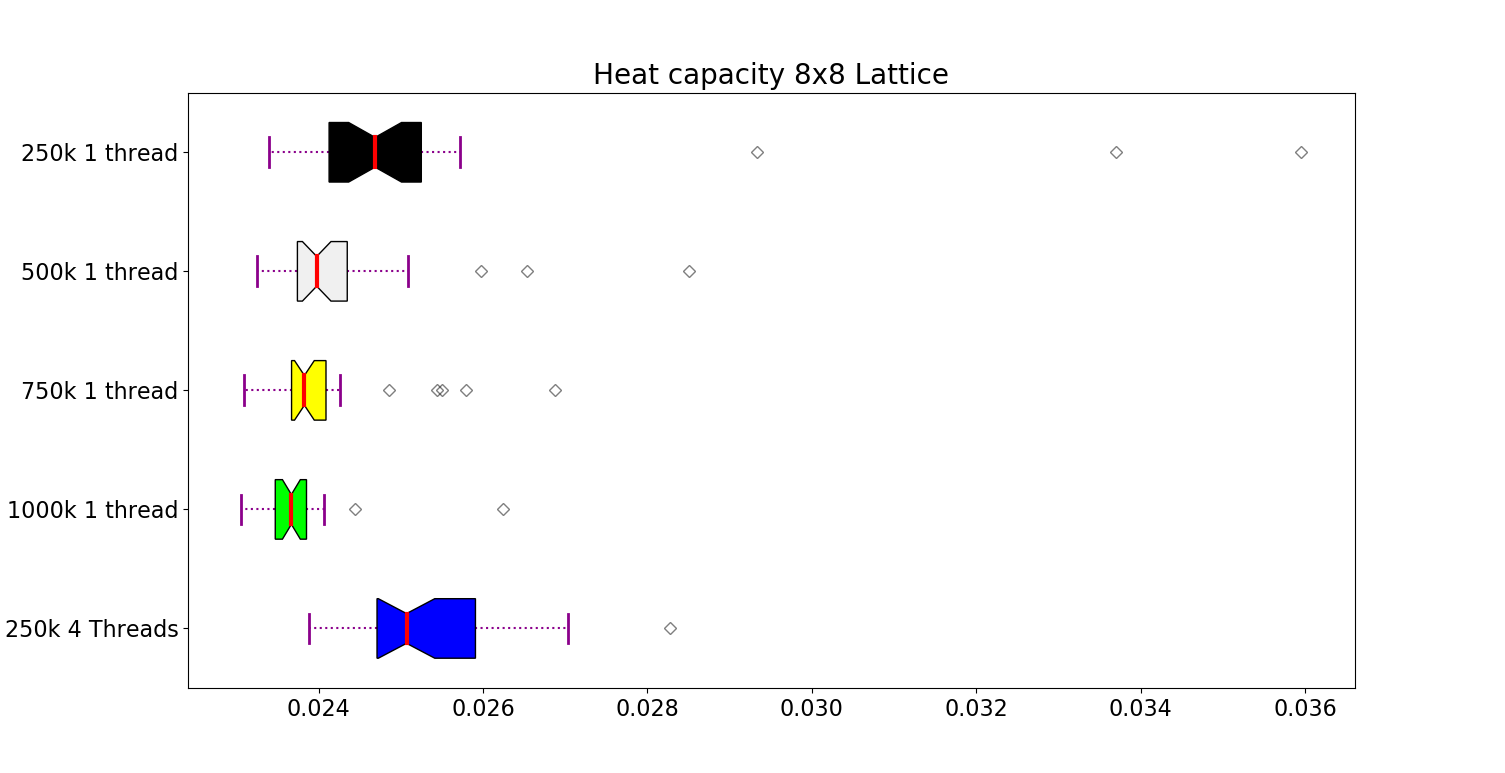
\includegraphics[width=1.0\textwidth]{Projects/P04/8x8_Cv.png}
%   \caption{8x8 Heat capacity.}
%   \label{8x8_Cv}
% \end{figure}
% \begin{figure}[H]
%   \centering
%   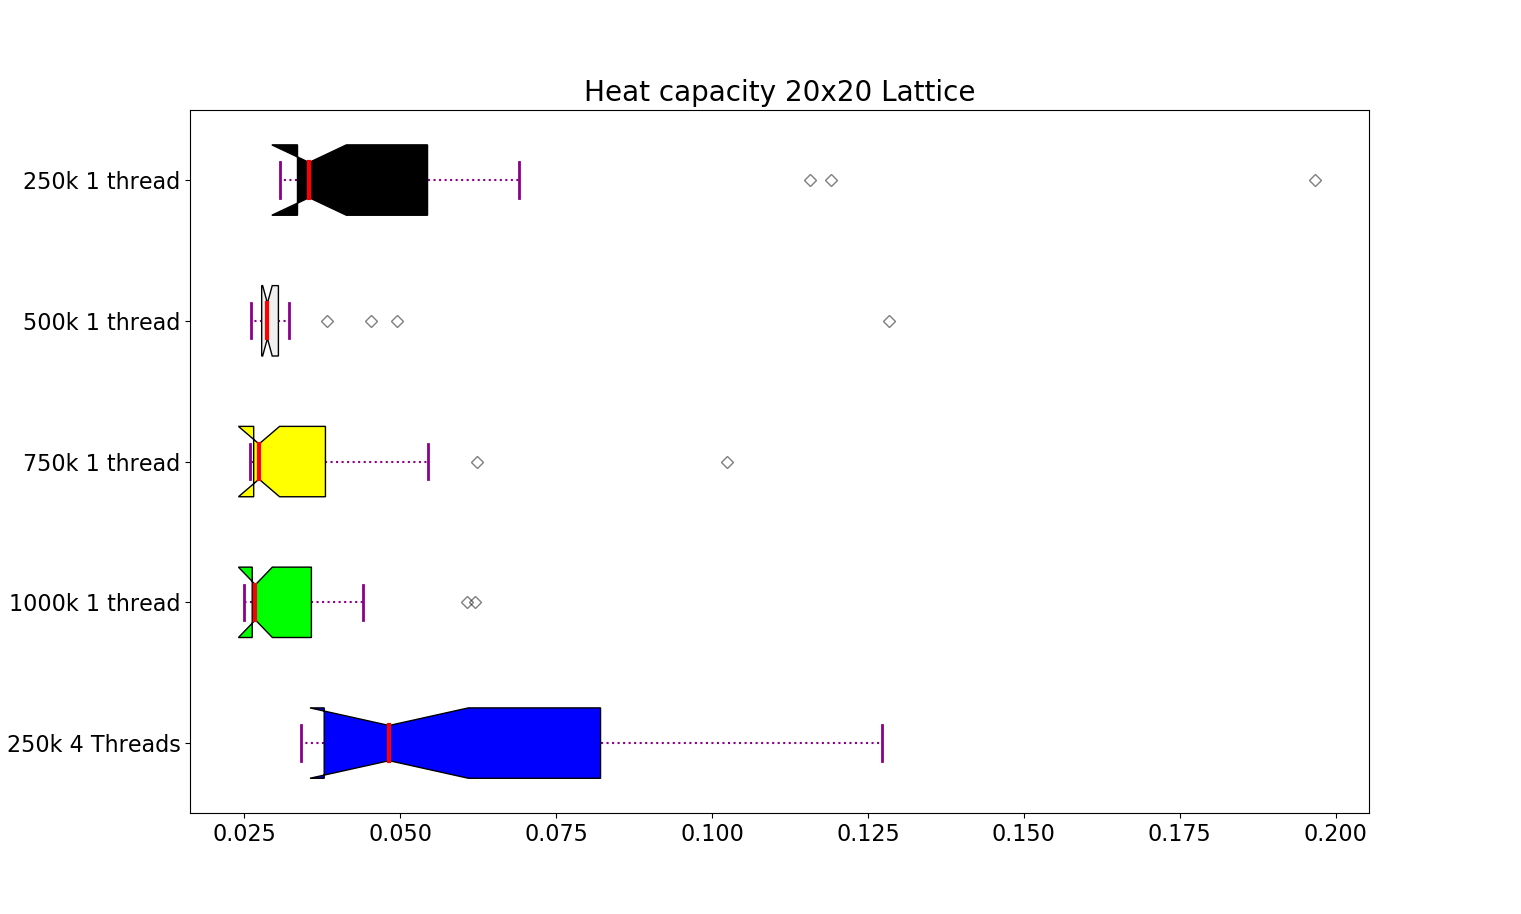
\includegraphics[width=1.0\textwidth]{Projects/P04/20x20_Cv.png}
%   \caption{20x20 Heat capacity.}
%   \label{20x20_Cv}
% \end{figure}


% \subsection*{Magnetic susceptibility}


% \begin{figure}[H]
%   \centering
%   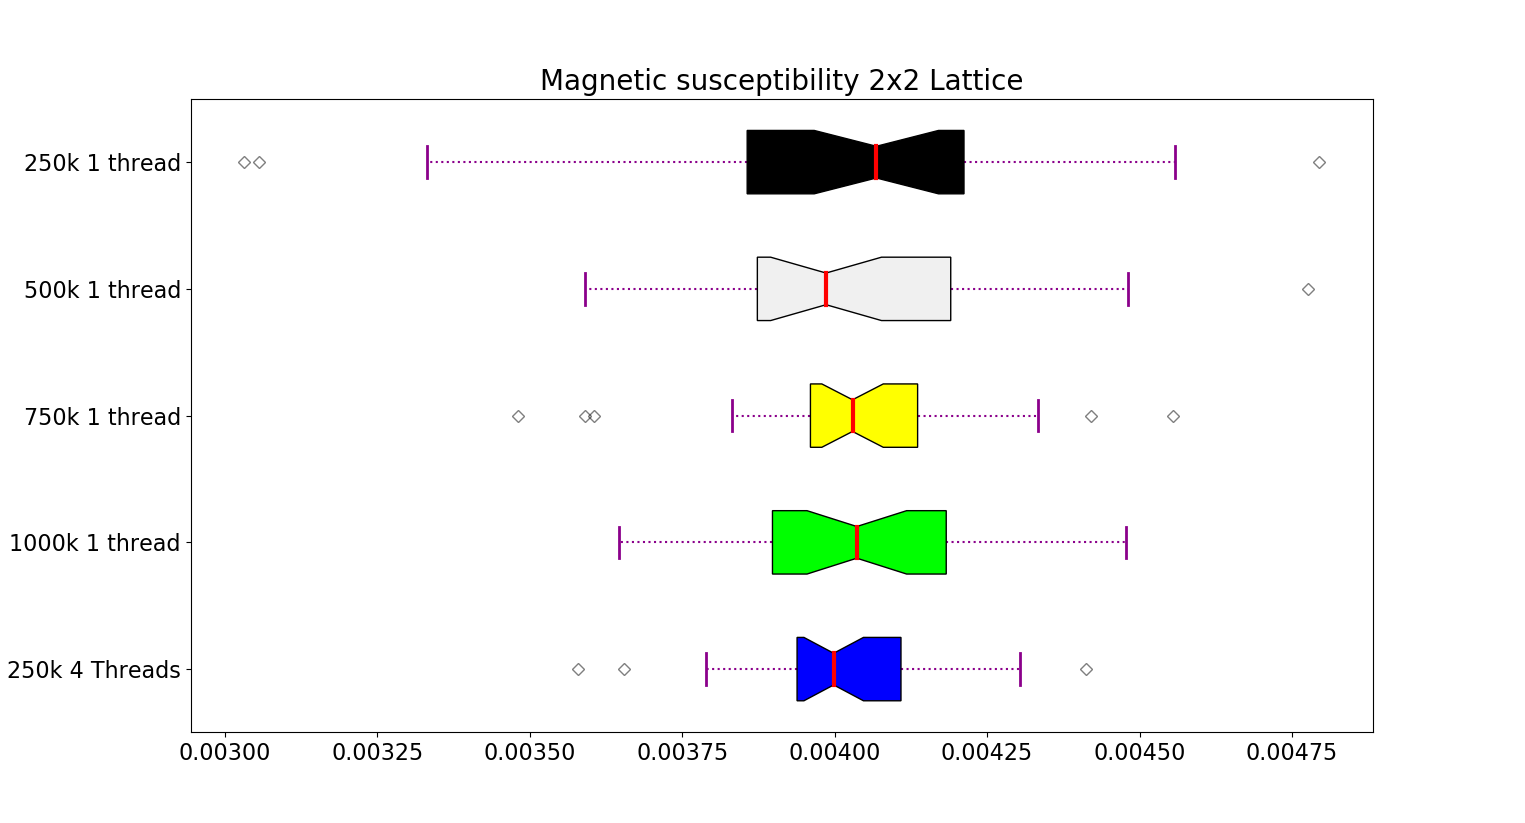
\includegraphics[width=1.0\textwidth]{Projects/P04/2x2_X.png}
%   \caption{2x2 Magnetic susceptibility.}
%   \label{2x2_X}
% \end{figure}
% \begin{figure}[H]
%   \centering
%   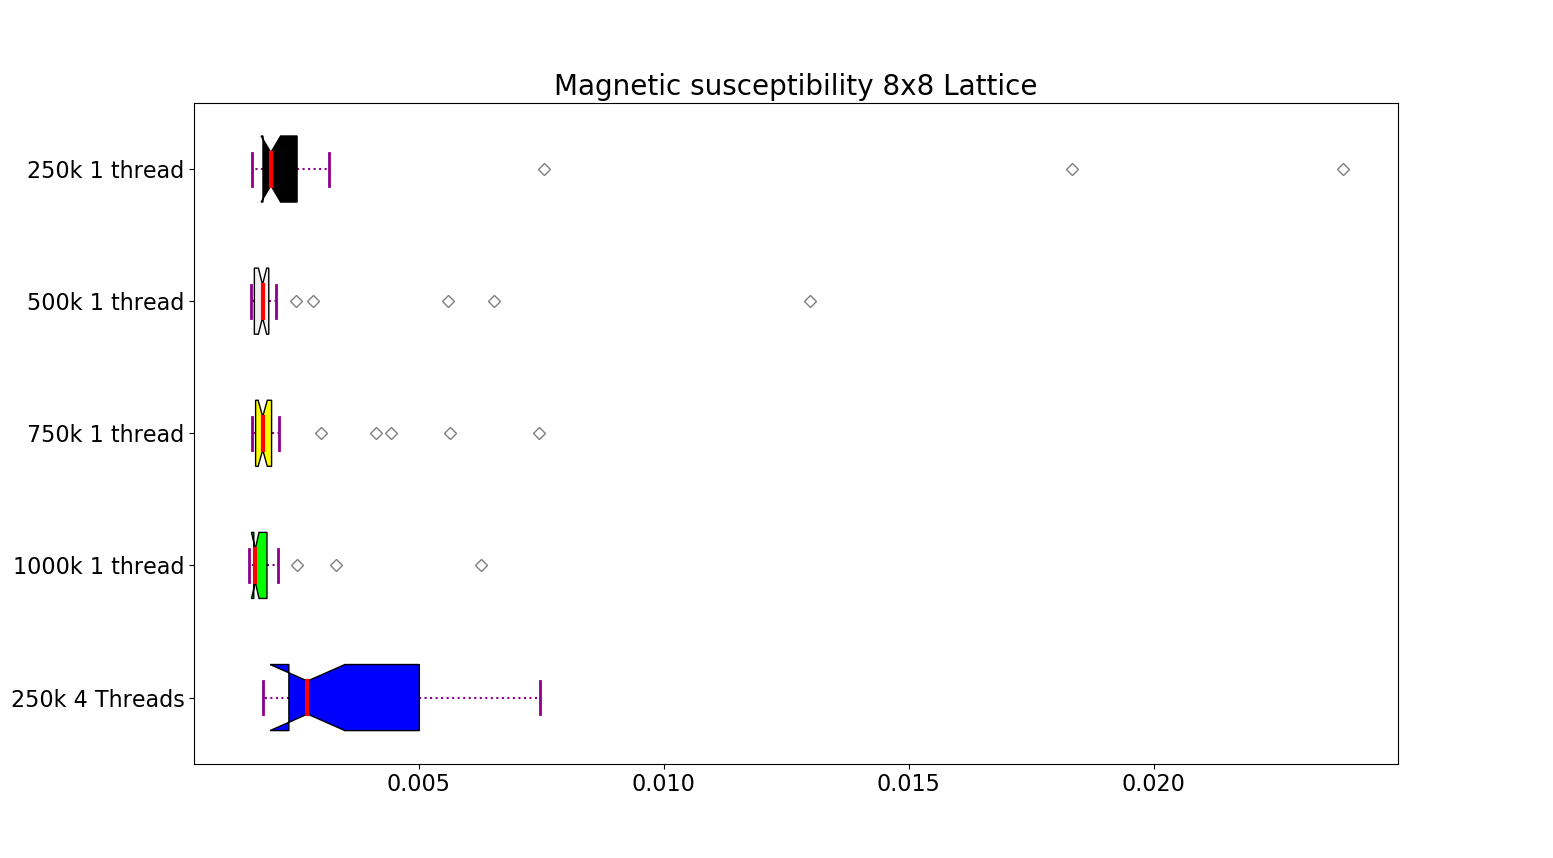
\includegraphics[width=1.0\textwidth]{Projects/P04/8x8_X.png}
%   \caption{8x8 Magnetic susceptibility.}
%   \label{8x8_X}
% \end{figure}
% \begin{figure}[H]
%   \centering
%   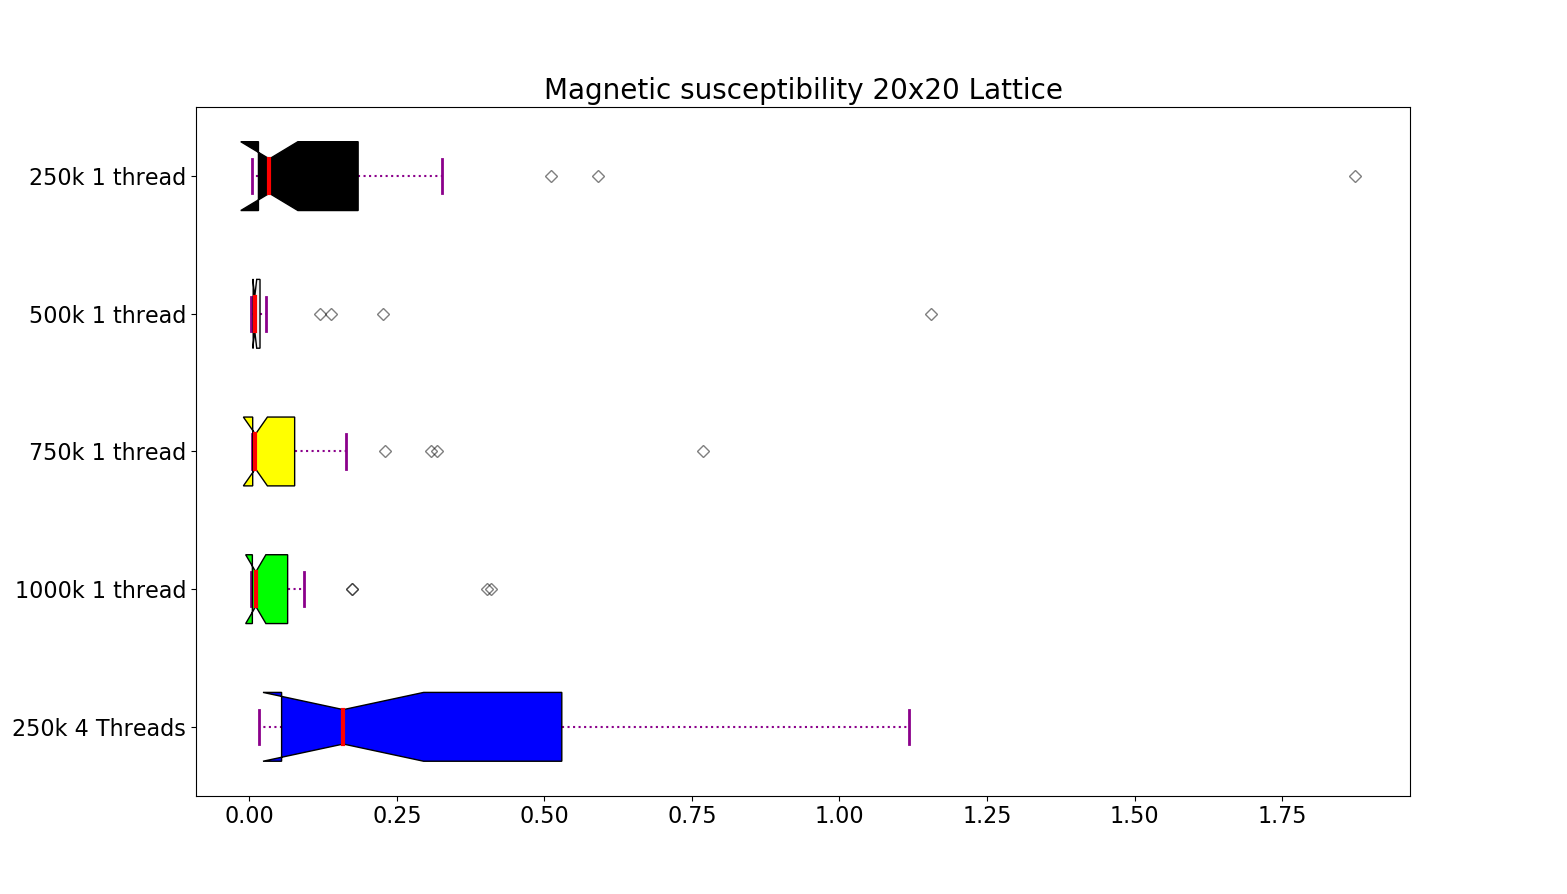
\includegraphics[width=1.0\textwidth]{Projects/P04/20x20_X.png}
%   \caption{20x20 Magnetic susceptibilityy.}
%   \label{20x20_X}
% \end{figure}



\end{appendix}
\end{document}
